\documentclass[11pt,compress,t,notes=noshow, aspectratio=169, xcolor=table]{beamer}

\usepackage{../../style/lmu-lecture}
% Defines macros and environments
% This file is included in slides and exercises

% Rarely used fontstyle for R packages, used only in 
% - forests/slides-forests-benchmark.tex
% - exercises/single-exercises/methods_l_1.Rnw
% - slides/cart/attic/slides_extra_trees.Rnw
\newcommand{\pkg}[1]{{\fontseries{b}\selectfont #1}}

% Spacing helpers, used often (mostly in exercises for \dlz)
\newcommand{\lz}{\vspace{0.5cm}} % vertical space (used often in slides)
\newcommand{\dlz}{\vspace{1cm}}  % double vertical space (used often in exercises, never in slides)
\newcommand{\oneliner}[1] % Oneliner for important statements, used e.g. in iml, algods
{\begin{block}{}\begin{center}\begin{Large}#1\end{Large}\end{center}\end{block}}

% Don't know if this is used or needed, remove?
% textcolor that works in mathmode
% https://tex.stackexchange.com/a/261480
% Used e.g. in forests/slides-forests-bagging.tex
% [...] \textcolor{blue}{\tfrac{1}{M}\sum^M_{m} [...]
% \makeatletter
% \renewcommand*{\@textcolor}[3]{%
%   \protect\leavevmode
%   \begingroup
%     \color#1{#2}#3%
%   \endgroup
% }
% \makeatother


\newcommand\tab[1][1cm]{\hspace*{#1}}
\tikzset{main node/.style={rectangle,draw,minimum size=1cm,inner sep=4pt},}

\usepackage[export]{adjustbox}
\usepackage[most]{tcolorbox}

\newtcolorbox{BlueBox}[2][]{%
   enhanced,
   colback   = blue!5!white,
   colframe  = blue!65!black,
   arc       = 1mm,
   outer arc = 1mm,
   fonttitle = \Large\slshape\textbf,
   center title,
   title     = #2,
   #1}

\title{Interpretable Machine Learning}
% \author{LMU}
%\institute{\href{https://compstat-lmu.github.io/lecture_iml/}{compstat-lmu.github.io/lecture\_iml}}
\date{}

\begin{document}

\newcommand{\titlefigure}{../../slides/01_intro/figure/open_blackbox}
\newcommand{\learninggoals}{
\item Introduction and Motivation
\item Dimensions of Interpretability
\item Bike Sharing Dataset}

\lecturechapter{Introduction to Interpretable Machine Learning}
\lecture{Interpretable Machine Learning}

\begin{frame}{Why Interpretability?}
% 		\begin{itemize}
% 			\item Machine learning (ML) has a huge potential to aid the decision-making process in various  applications.
% 			\pause
% 			\smallskip
% 			\item ML models often are intransparent black boxes, e.g., XGBoost, RBF SVM, or NNs.
% 			\begin{itemize}
% 				\item[$\rightarrow$] too complex to be understood by humans.
% 			\end{itemize}
% 			\smallskip
% 			\item A lack in explanations diminishes trust in the model and creates barriers for adoption, especially in areas with critical decision-making consequences, e.g., medicine.
% 			\smallskip
% 			\item Such disciplines often rely on traditional models,\\ e.g., linear models, with less predictive performance.
% 			\smallskip
% 			\item Interpretable machine learning (IML) aims to bridge the gap between interpretability and predictive performance.
% 		\end{itemize}
\bigskip
    \begin{columns}[T, totalwidth=\textwidth]
    \begin{column}{0.8\textwidth}
		\begin{itemize}
			\item ML: huge potential to aid decision-making process due to its predictive performance
			%\pause
			%\smallskip
			\item ML models are often black boxes, e.g., XGBoost, RBF SVM or DNNs
			\begin{itemize}
				\item[$\leadsto$] too complex to be understood by humans
			\end{itemize}
			%\pause
			%\smallskip
			\item Lack of explanation
			\begin{enumerate}
				\item hurts trust
				\item creates barriers
			\end{enumerate}
		\item[$\leadsto$] Harder to adapt for critical areas with decisions affecting human life
			\item[\,$\leadsto$] Many disciplines with required trust rely on traditional models,\\ e.g., linear models, with less predictive performance
		\end{itemize}
	\end{column}
	\begin{column}{0.2\textwidth}  %%<--- here
        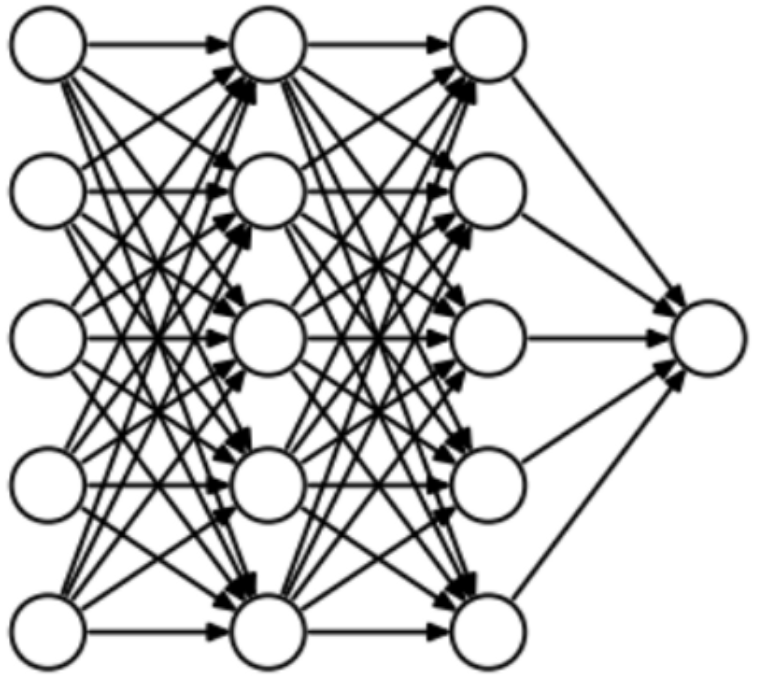
\includegraphics[width=0.9\textwidth]{../../slides/01_intro/figure/nn_model.png}
        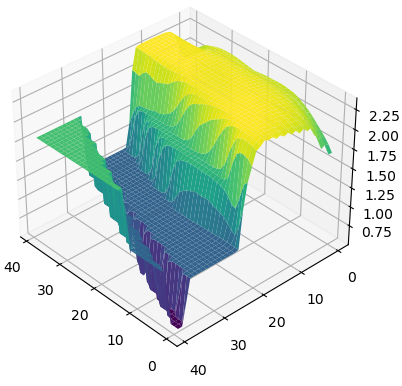
\includegraphics[width=0.9\textwidth]{../../slides/01_intro/figure/nn_landscape.png}
        \centering \citebutton{Liu 2021}{https://davideliu.com/2021/12/12/visualizing-loss-landscape-of-gail/}
    \end{column}
    \end{columns}
    % \bigskip
    % \begin{columns}[T, totalwidth=\textwidth]
    %     \begin{column}{0.5\textwidth}
    %     \begin{itemize}
    %         \only<5>{\item[$\leadsto$] Harder to adapt for critical areas with decisions affecting human life}
    %         \item<5>[\,$\leadsto$] Many disciplines with required trust rely on traditional models,\\ e.g., linear models, with less predictive performance
    %     \end{itemize}
    %     \end{column}
	   % \begin{column}{0.5\textwidth} 
	   %     \only<5>{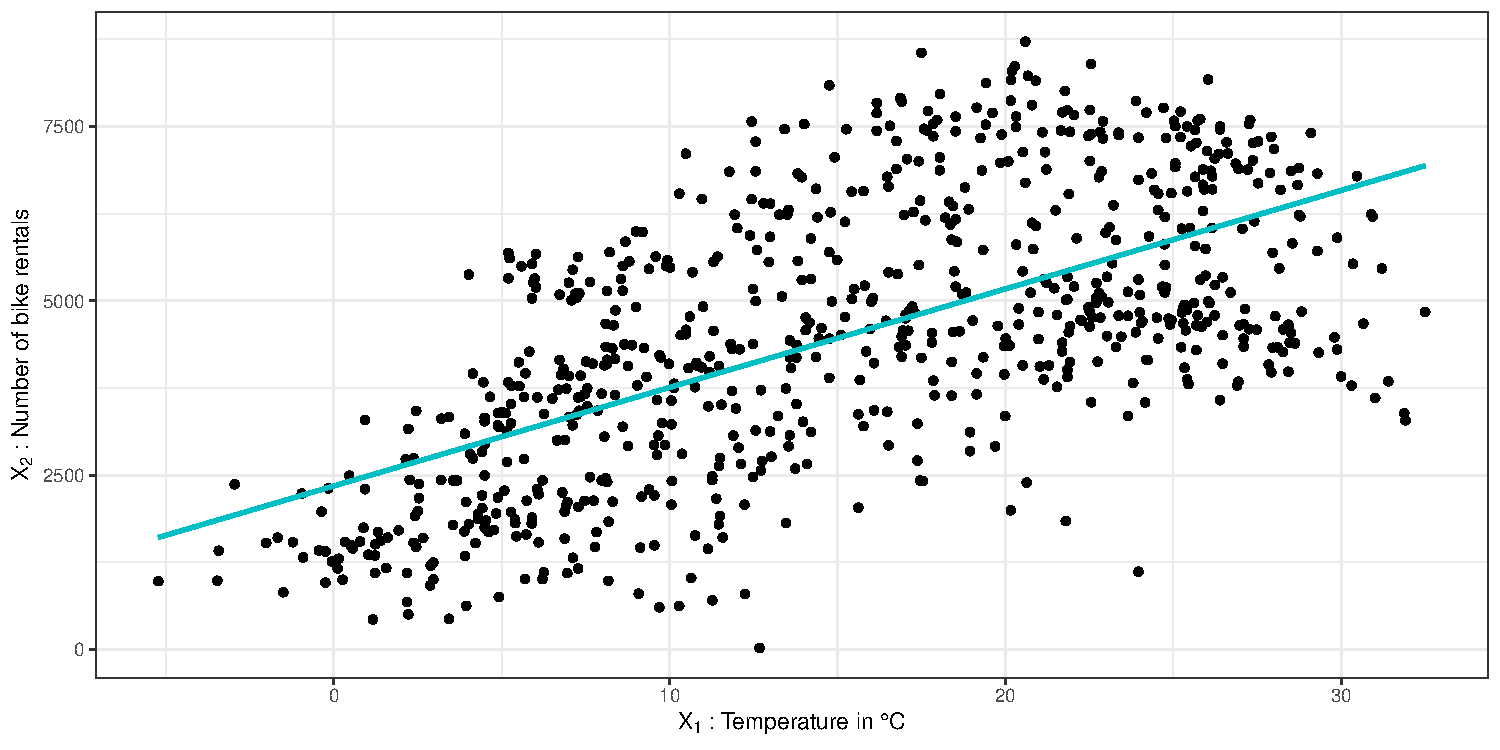
\includegraphics[width=\textwidth]{figure/intro_lm_bike.pdf}}
	   % \end{column}
    %     \end{columns}
\end{frame}
	
	
% \begin{frame}{Need for Interpretability in High-stakes Decisions}

% Examples of critical areas where decisions based on ML models can affect human life 
%     % \begin{itemize}
%     %     \item Credit scoring and insurance applications
%     %     \citebutton{Society of Actuaries}{https://www.soa.org/resources/research-reports/2021/interpretable-machine-learning}
%     % \end{itemize}
%     \begin{columns}[T, totalwidth=\textwidth]
%     \begin{column}{0.55\textwidth}
% 		\begin{itemize}
% 		\item Credit scoring and insurance applications
%         \citebutton{Society of Actuaries}{https://www.soa.org/resources/research-reports/2021/interpretable-machine-learning}
%         \begin{itemize}
%             \item Providing reasons for not granting a loan
%             \item Fraud detection in insurance claims
%         \end{itemize}
%         \item<2-> Medical applications
%         \begin{itemize}
%             \item Identification of diseases
%             \item Chance of recovering
%             \item Recommendations of treatments
%         \end{itemize}
%         \item<2-> \ldots
%     \end{itemize}
%     \end{column}
% 	\begin{column}{0.45\textwidth}
%         \includegraphics<1->[page=1, width=\textwidth, trim = 0 250 0 0, clip]{../../slides/01_intro/figure/counterfactual.pdf}
%         \medskip
% 	    \only<2->{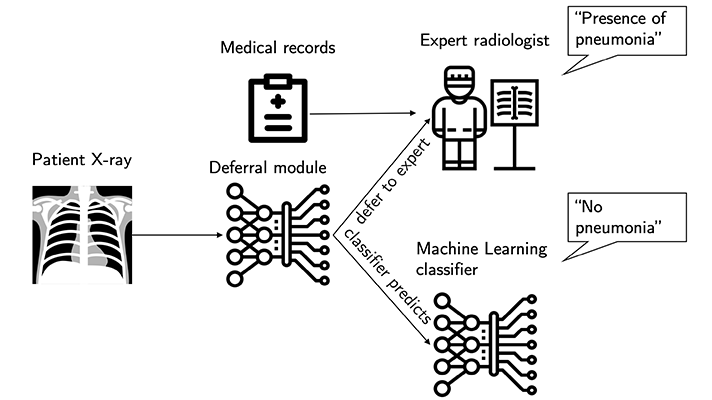
\includegraphics[width=\textwidth]{../../slides/01_intro/figure/medicine.png}
% 	    \centering \citebutton{Miliard (2020)}{https://www.healthcareitnews.com/news/new-ai-diagnostic-tool-knows-when-defer-human-mit-researchers-say}}
% 	\end{column}
%     \end{columns}
% \end{frame}


\begin{frame}{Need for interpretability in High-stakes Decisions}

    Need for interpretability also becoming increasingly important from a legal perspective
    
    \begin{itemize}
    \item General Data Protection Regulation (GDPR) requires for some applications that models have to be explainable \citebutton{Goodman \& Flaxman (2017)}{https://doi.org/10.1609/aimag.v38i3.2741}\\
    $\leadsto$ \textit{EU Regulations on Algorithmic Decision-Making and a ``Right to Explanation''} 
    
    \item \textit{Ethics guidelines for trustworthy AI}
    \citebutton{European Commission (2019)}{https://doi.org/10.2759/346720}

    \end{itemize}
    \medskip
    
    \centering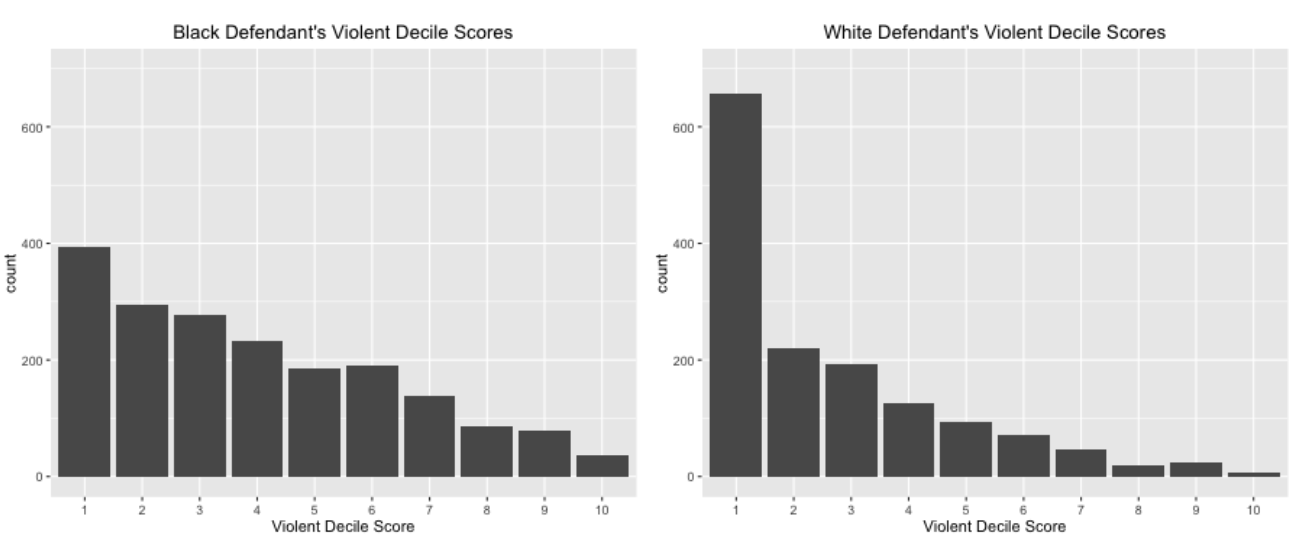
\includegraphics[width=0.7\textwidth]{../../slides/01_intro/figure/compass_black_white.PNG}
    % source https://www.propublica.org/article/how-we-analyzed-the-compas-recidivism-algorithm
\end{frame}


	%-----------------------------------------------------------------------------------------------------------------------------

% \begin{frame}{Brief History of Interpretability}
% 	\begin{columns}[T, totalwidth=\textwidth]
% 	\begin{column}{0.75\textwidth}
% 	    \begin{itemize}
% 			\item 18th and 19th century: \\linear regression models (Gauss, Legendre, Quetelet)
% 			\medskip
% 			\item<2-> 1940s:\\ emergence of sensitivity analysis (SA)
% 			\medskip
% 			\item<3-> Middle of 20th century:\\ Rule-based ML, incl. decision rules and decision trees
% 			\medskip
% 			\item<4-> 2001:\\ built-in feature importance measure of random forests
% 			\medskip
% 			\item<5-> >2010: \\Explainable AI (XAI) for deep learning
% 			\medskip
% 			\item<6> >2015: \\IML as an independent field of research
% 		\end{itemize}
% 	\end{column}
% 	\begin{column}{0.25\textwidth}
% 	    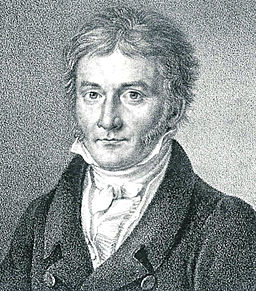
\includegraphics[width=0.8\textwidth]{../../slides/01_intro/figure/Carl_Friedrich_Gauss_1828.jpg}
%         \centering \citebutton{Carl Friedrich Gauss}{https://commons.wikimedia.org/w/index.php?curid=2404149}
%         \centering \citebutton{Wikipedia}{https://en.wikipedia.org/wiki/Carl_Friedrich_Gauss}
%         \bigskip\\
%         \only<3->{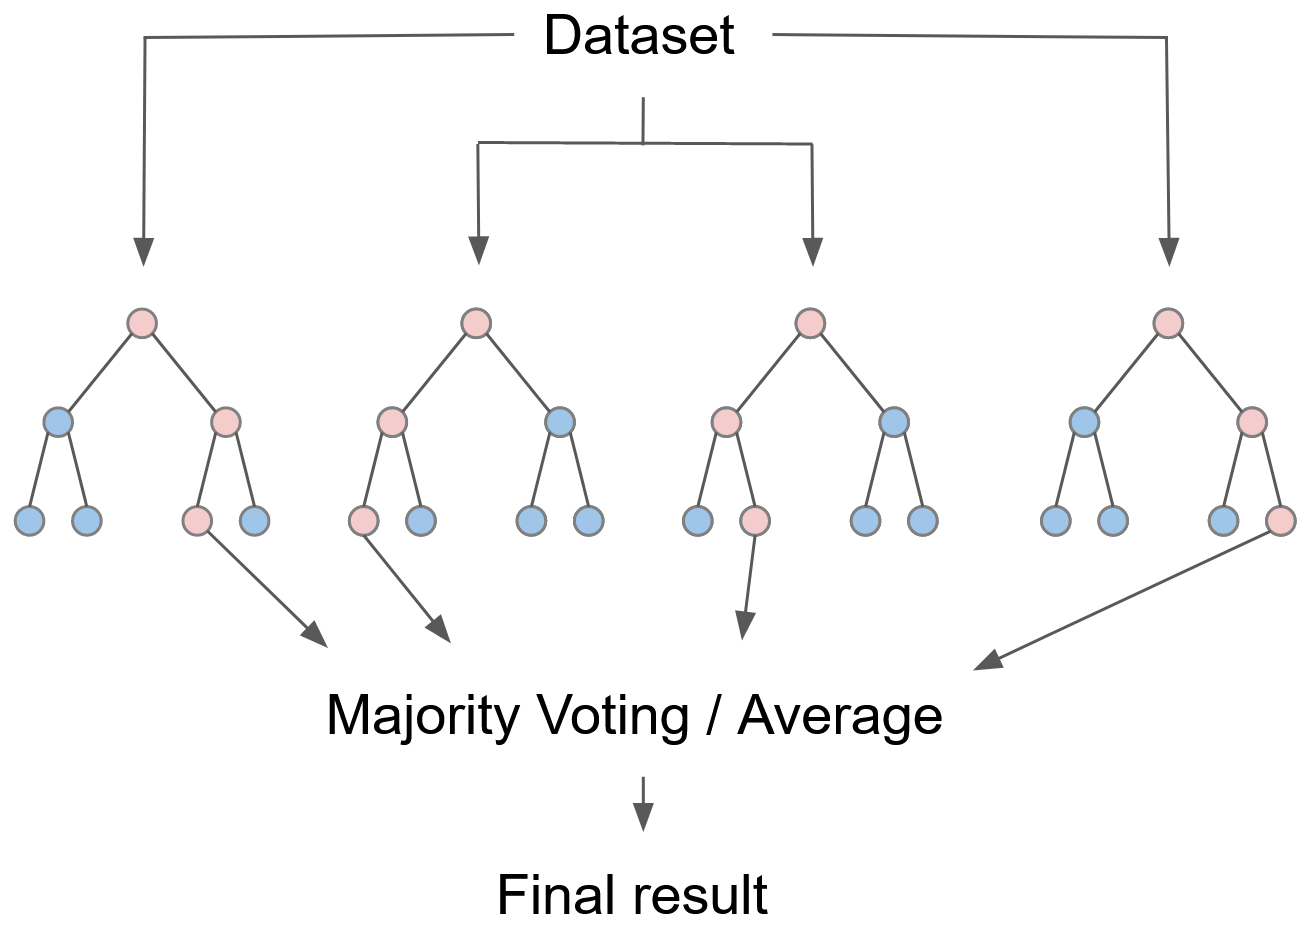
\includegraphics[width=0.9\textwidth]{../../slides/01_intro/figure/Random_Forest.png}}
%         % https://docs.google.com/presentation/d/15HjwMHdTtZ9N0cniUPsiztRSRg1UDY3Y5M8tXsaqt2I/edit?usp=sharing
% 	\end{column}
% 	\end{columns}
% \end{frame}

	%-----------------------------------------------------------------------------------------------------------------------------
% \begin{frame}{When do we need interpretability?}
% \begin{columns}[T, totalwidth=\textwidth]
% \begin{column}{0.6\textwidth}
% %  \begin{itemize}
% %   \item Debugging machine learning models
% %   \item Increasing trust in models
% %   \item Analyzing newly developed systems with unknown consequences
% %   \item Decisions about humans
% %   \item Models using proxies instead of causal inputs, e.g. predicting flu outbreaks from google searches.
% %   \item When loss function does not cover constraints like fairness (e.g. credit score) or need for insights (e.g. science).
% % \end{itemize}
% \begin{itemize}
%   \item To \textbf{Discover}: Gain insights about data, distribution and model
%   \pause 
%   \item To \textbf{Debug, audit and improve}: Insights help to identify flaws (in data or model), which can be corrected (debug and audit)\\
%   $\leadsto$ Global perspective
%   \pause
%   \item To \textbf{explain individual decisions}: Explaining individual decisions can prevent unwanted actions based on the model\\
%   $\leadsto$ Local perspective
%   \pause 
%   \item To \textbf{Justify}: Investigate if and why biased, unexpected or discriminatory predictions were made, or improve/reject the model\\
%   $\leadsto$ Fairness perspective

% \end{itemize}
% \end{column}
% \begin{column}{0.4\textwidth}  %%<--- here
%  %\vspace{0.5cm}
% %  \begin{center}
% %  \begin{figure}
%   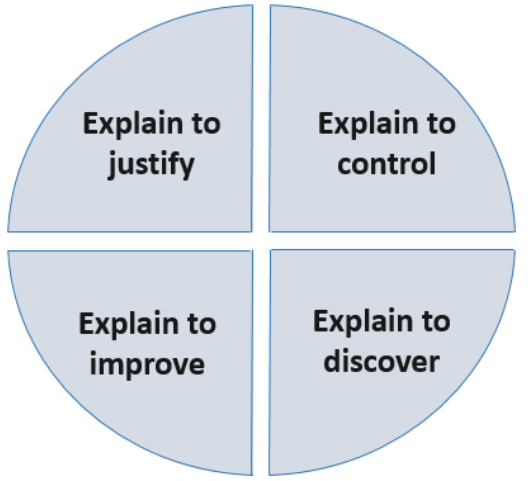
\includegraphics[width=0.9\textwidth]{figure/explain-to}
%   \centering \citebutton{Adadi and Berrada 2018}{https://doi.org/10.1109/ACCESS.2018.2870052}
% %  \end{figure}
% %  \end{center}
% \end{column}
% \end{columns}
%      %\lz
%     %\footnote[frame]{Doshi-Velez, F., \& Kim, B. (2017). Towards A Rigorous Science of Interpretable Machine Learning. arXiv: 1702.08608.}
%     %\footnote[frame]{A. Adadi and M. Berrada, "Peeking Inside the Black-Box: A Survey on Explainable Artificial Intelligence (XAI)," in IEEE Access, vol. 6, pp. 52138-52160, 2018.}
% \end{frame}

\begin{frame}{When do we need interpretability}

% \begin{columns}[T, totalwidth=\textwidth]
  %   \begin{column}{0.8\textwidth}
		\begin{center}
            \def\firstcircle{(90:1cm) circle (2.5cm)}
            \def\secondcircle{(210:2.5cm) circle (2.5cm)}
            \def\thirdcircle{(330:2.5cm) circle (2.5cm)}
            \def\fourthcircle{(90:-3.5cm) circle (2.5cm)}
            \resizebox{6.5cm}{6.5cm}{
            \begin{tikzpicture}
                \begin{scope}[ fill opacity=0.5]
                    \fill[red] \firstcircle;
                    \fill[green] \secondcircle;
                    \fill[blue] \thirdcircle;
                    \fill[cyan] \fourthcircle;
                \end{scope}
                \draw \firstcircle node[text=black,above, text width=2cm, align=center] {Discover and global insights};
                \draw \secondcircle node [text=black, left, text width=2cm, align=center] {Improve model, debug and audit};
                \draw \thirdcircle node [text=black,right, text width=2cm, align=center] {Understand and control individual predictions};
                \draw \fourthcircle node [text=black,below, text width=2cm, align=center]{Justification and fairness};
            \end{tikzpicture}}
        \end{center}
 %    \end{column}
	% \begin{column}{0.2\textwidth}
 %        \centering \citebutton{Miliard (2020)}{https://www.healthcareitnews.com/news/new-ai-diagnostic-tool-knows-when-defer-human-mit-
	% \end{column}
 %    \end{columns}

\footnote[frame]{A related presentation can be found in \citebutton{Adadi and Berrada 2018}{https://doi.org/10.1109/ACCESS.2018.2870052}.}

\end{frame}



% \begin{frame}{Why is Interpretability Important?}

% 	\begin{itemize}
% 	    \item Machine learning is (mostly) about discovering patterns in data.
% 	    \medskip
% 	    \item Unfortunately, it is not guaranteed that ML will identify the correct patterns.

% 	    \medskip
% 	    \item We humans might not be able to discover patterns ML models discovered.
% 	    \begin{itemize}
% 	        \item Good for science or to get new insights.
% 	        \item Bad in applications where unexpected behavior is not desired.
% 	    \end{itemize}
% 	    \medskip

% 	    \item \alert{How can you check whether the model is correct in its inference?}
% 	\end{itemize}

% \end{frame}

\begin{frame}{Discover and global insights}
$\leadsto$ Gain insights about data, distribution and model \\
\medskip
\textbf{Example:} Bike Sharing Dataset (predict number of bike rentals per day) \\
\textit{Exemplary question:} Which feature influences the model performance and to what extent?
\begin{center}
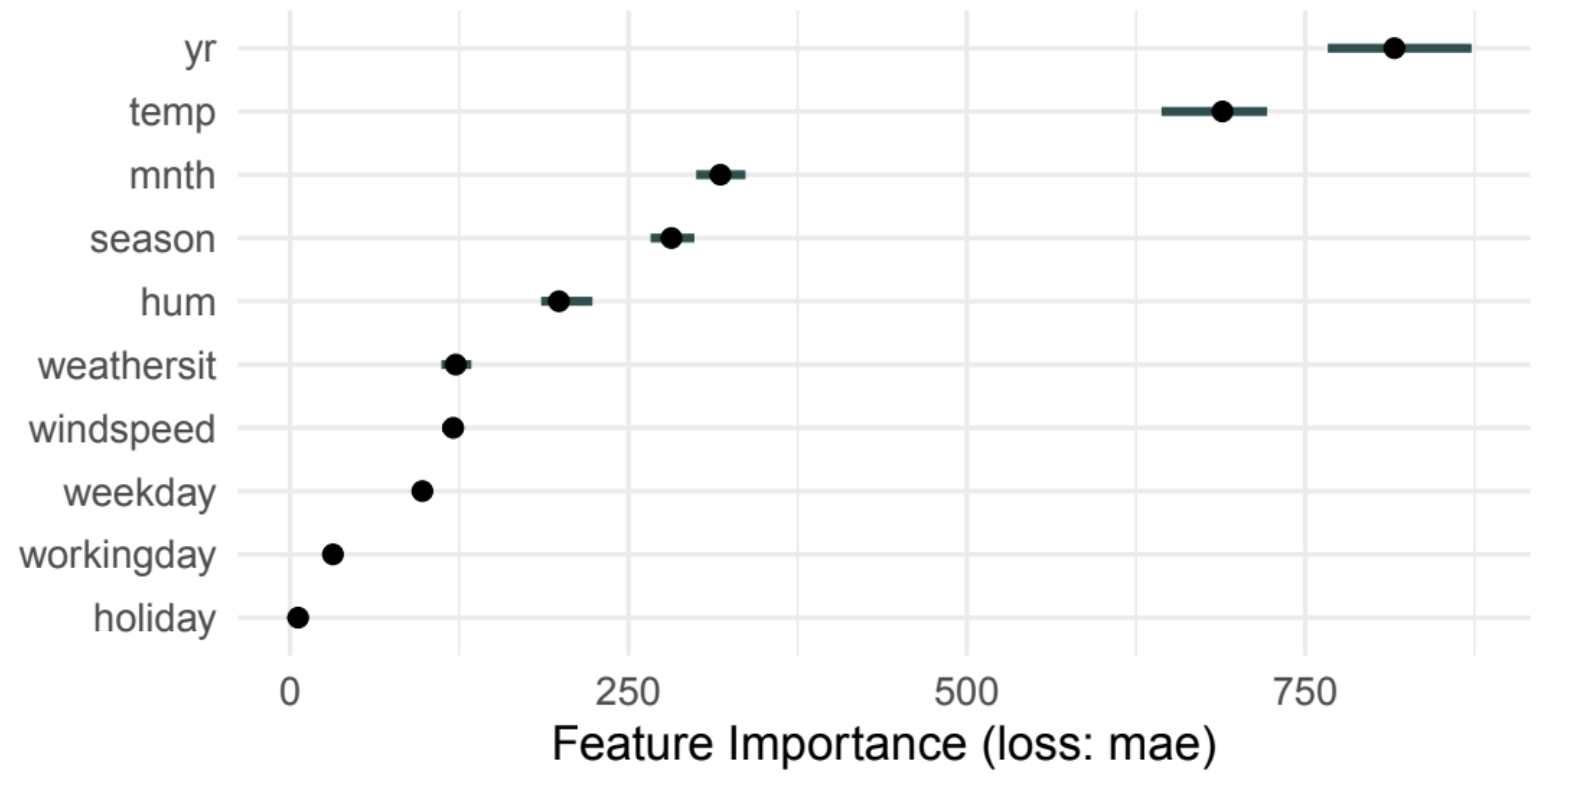
\includegraphics[width=0.6\textwidth]{../../slides/01_intro/figure/bike-sharing02.png}
\end{center}

%\textbf{Interpretation:}

\begin{itemize}
    \item Year (\code{yr}) and Temperature (temp) most important features
    \item Holiday (\code{holiday}) less important (Can we drop it?)
\end{itemize}

\end{frame}

% \begin{frame}{Example (Improve model, debug and audit): Clever Hans \citebutton{Lapuschkin et al. 2019}{https://www.nature.com/articles/s41467-019-08987-4} }

% 	\centering
% 	\begin{columns}[T, totalwidth=\textwidth]
% 	\begin{column}{0.6\textwidth}
% 	\includegraphics<1>[width=\textwidth]{figure/horse_without_label.PNG}
% 	\includegraphics<2>[width=\textwidth]{figure/horse_with_label.PNG}
% 	\includegraphics<3>[width=\textwidth]{figure/horse_map_with_label.PNG}
% 	\includegraphics<4>[width=\textwidth]{figure/horse_map_without_label.PNG}
% 	\end{column}
% 	\begin{column}{0.4\textwidth}

% 	\begin{itemize}
% 	    \item Horse with claimed math skills
% 	    \item Answered questions correctly by hoof tapping or head shaking
% 	    \item Correct answers were traced to involuntary cues from human's body language $\Rightarrow$ no math skills %asking person
% 	    %(e.g., tense attitude)
% 	    \item<2-> Image classification: \\
% 	    source tag present \\
% 	    \onslide<3->{$\Rightarrow$ classified as horse}
% 	    \item<4-> no source tag \\ $\Rightarrow$ not classified as horse
% 	\end{itemize}

% 	\end{column}
% 	\end{columns}
% \end{frame}

\begin{frame}{Improve model, debug and audit}
$\leadsto$ Insights help to identify flaws (in data or model), which can be corrected \\
\medskip
\textbf{Example:} Neural Net Tank \citebutton{gwern.net}{https://www.gwern.net/Tanks} \\
	\centering
	\begin{columns}[T, totalwidth = \textwidth]
	\begin{column}{0.44\textwidth}
	\centering
	% pictures from pixabay
	\only<1>{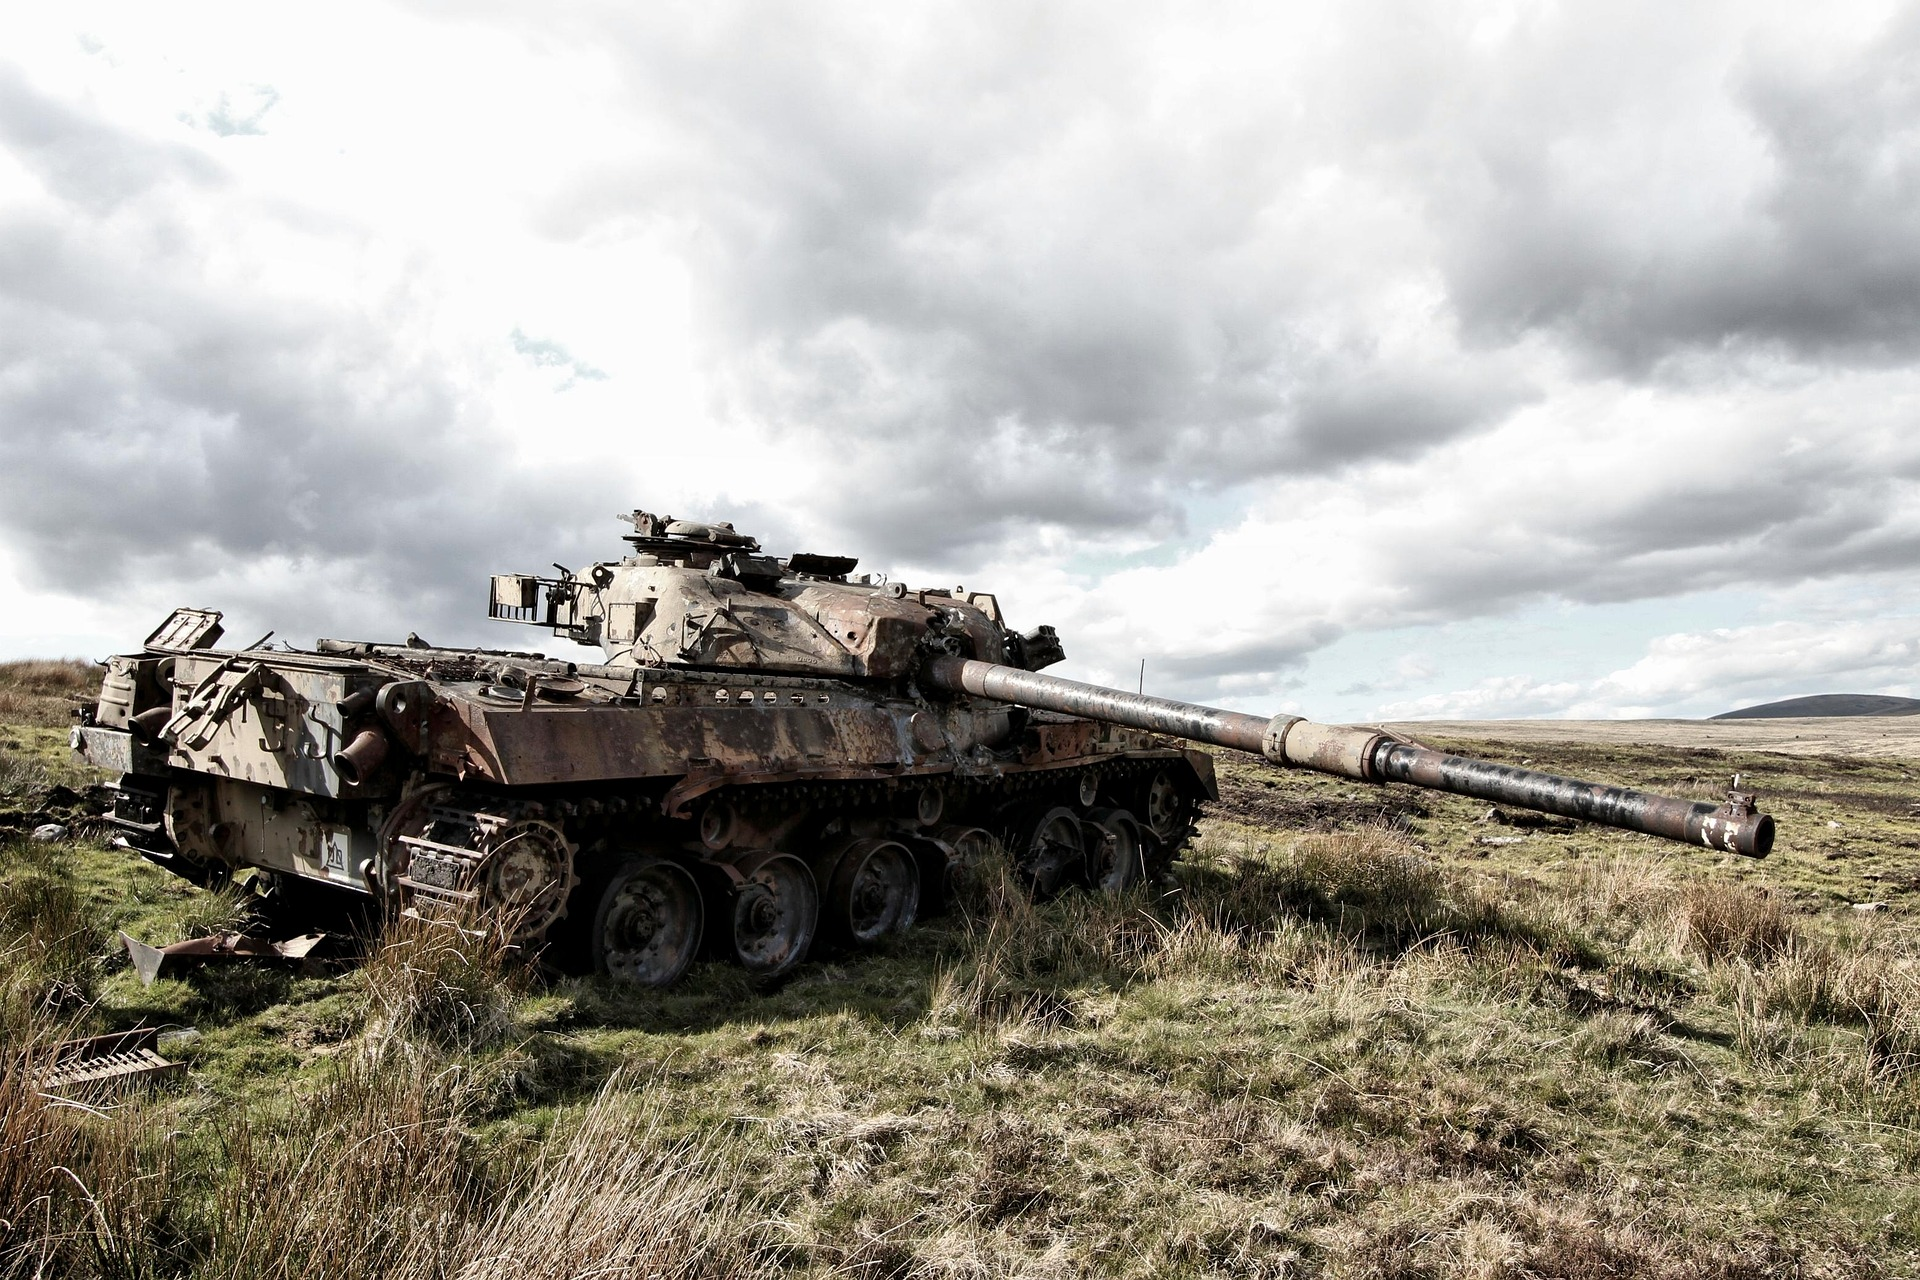
\includegraphics[width=\textwidth]{../../slides/01_intro/figure/tank.jpg}}
	\only<2>{
        \begin{figure}
            \centering
            \begin{tabular}{@{}c@{}}
                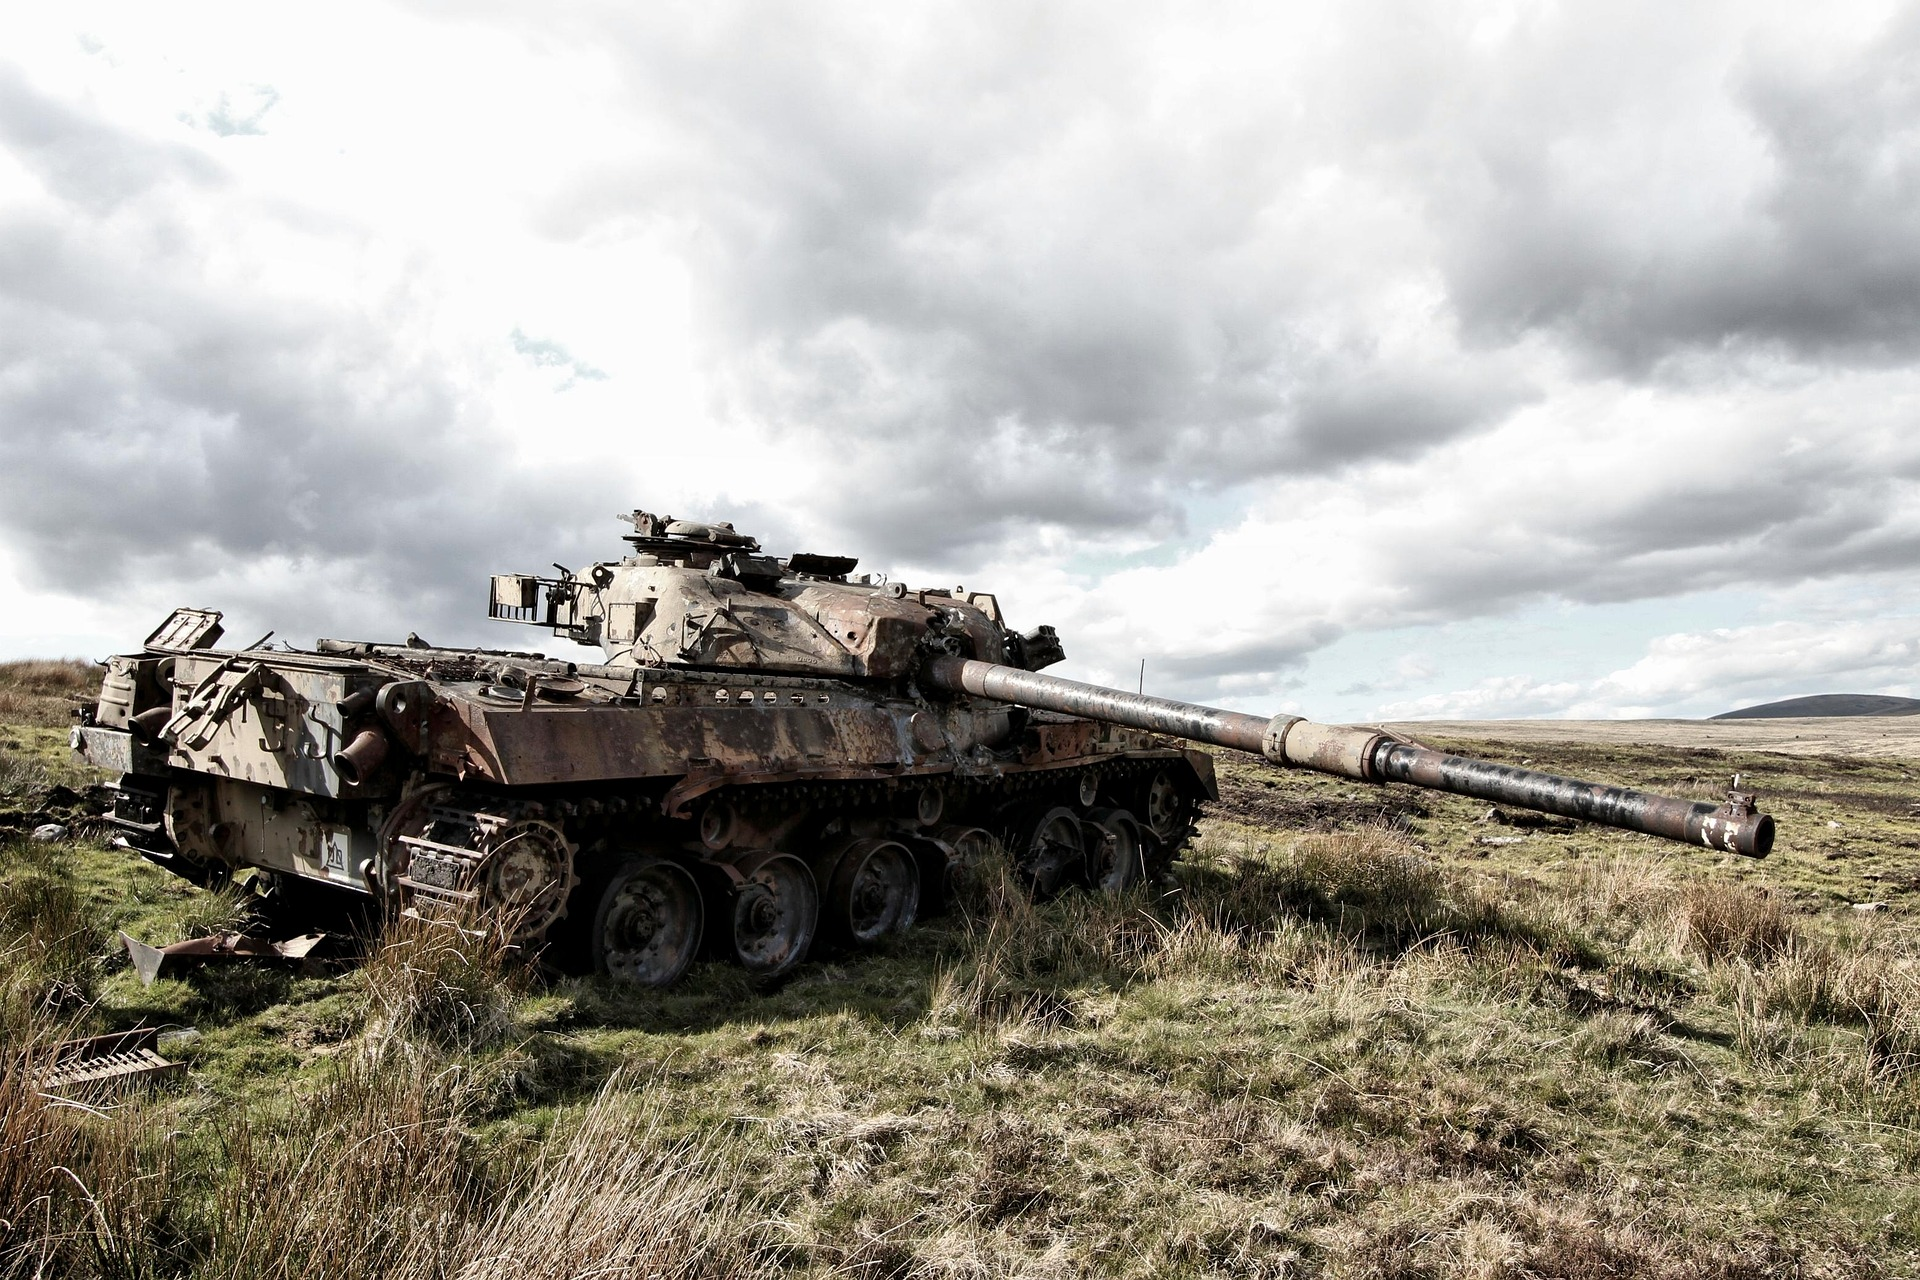
\includegraphics[width=0.65\textwidth]{../../slides/01_intro/figure/tank.jpg}
            \end{tabular}

            \begin{tabular}{@{}c@{}}
        	    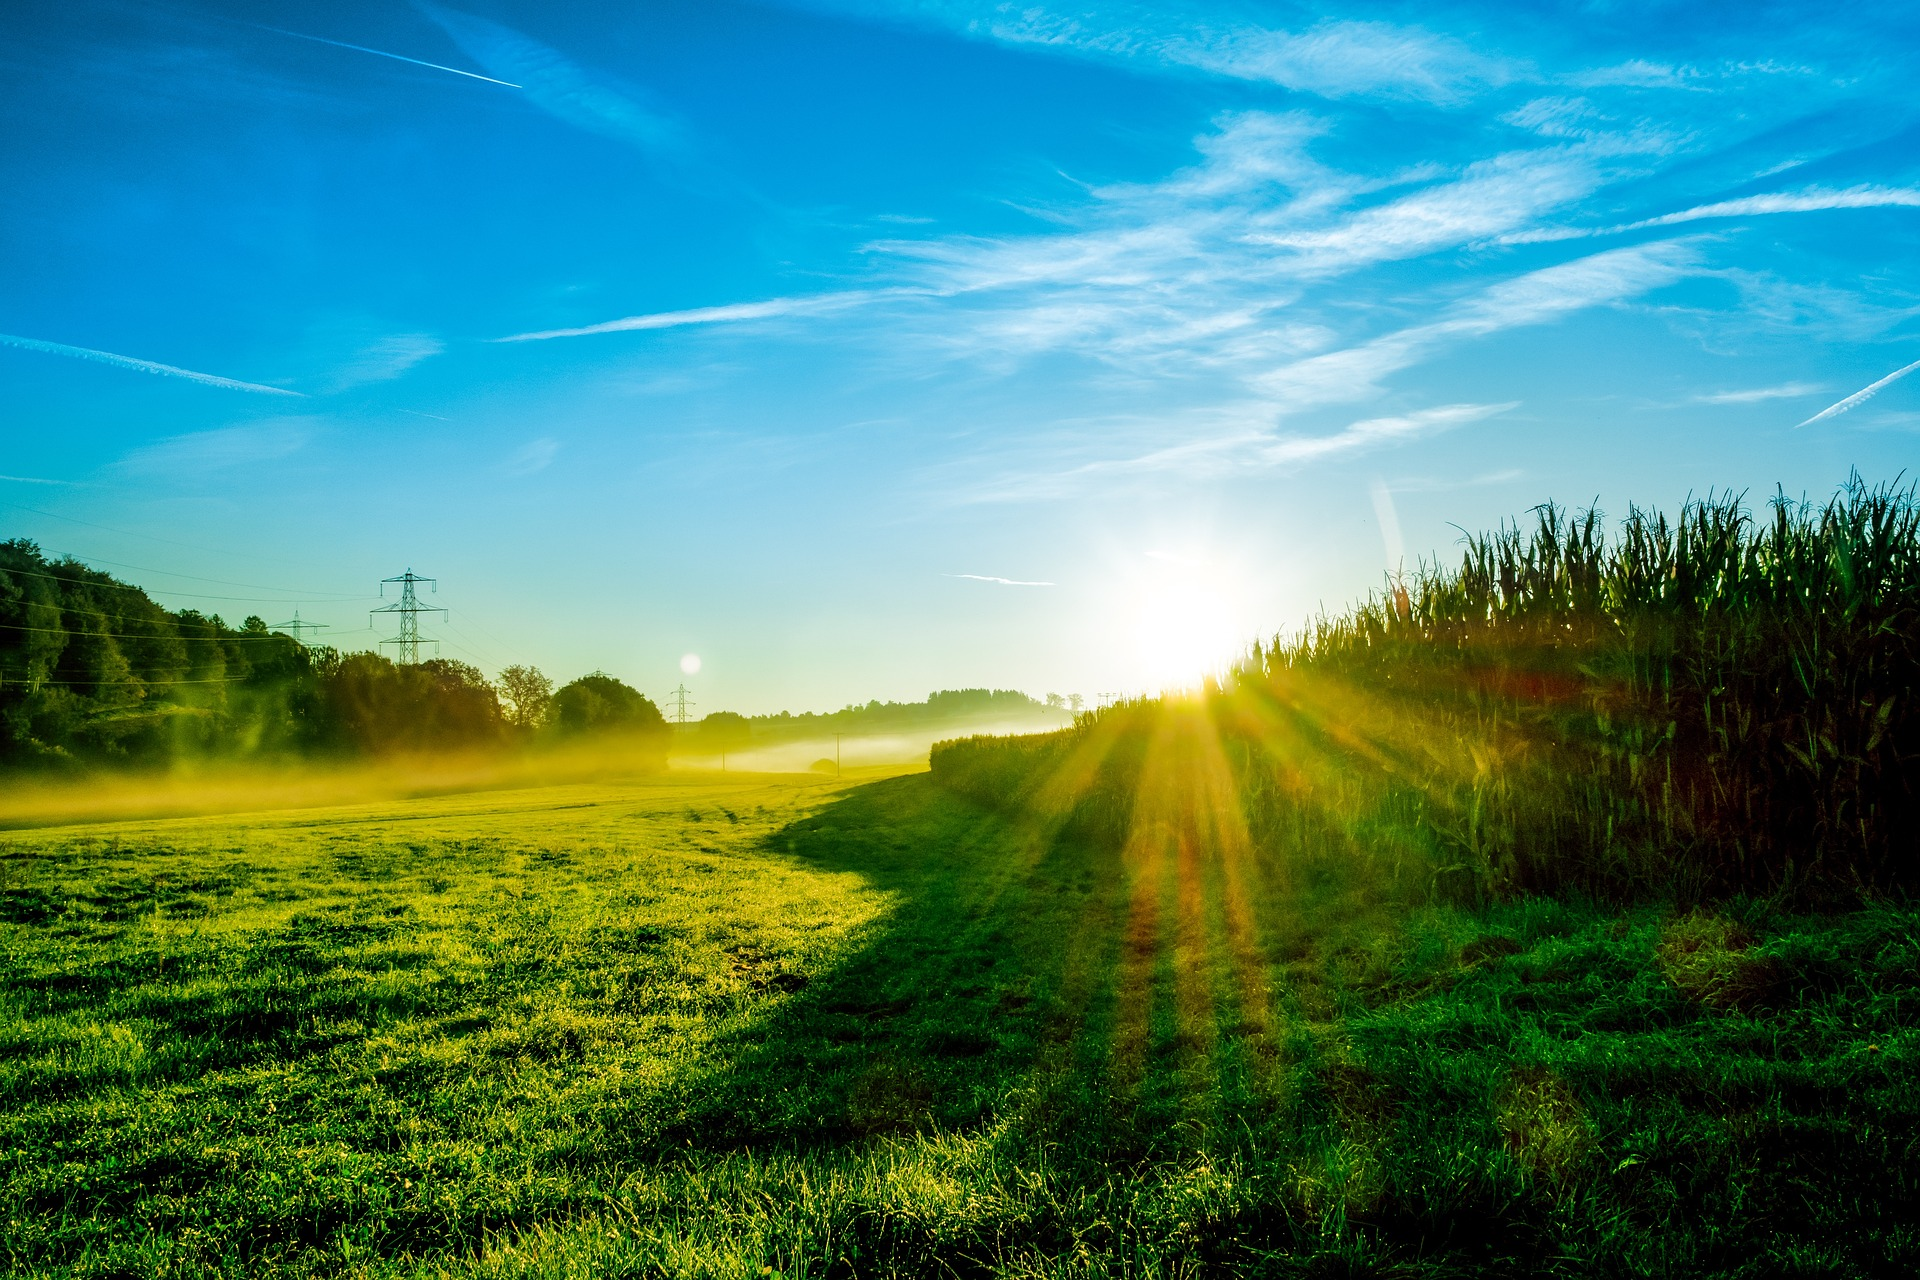
\includegraphics[width=0.65\textwidth]{../../slides/01_intro/figure/landscape.jpg}
            \end{tabular}
        \end{figure}
    }
    \only<3>{\vspace{0.7cm}
            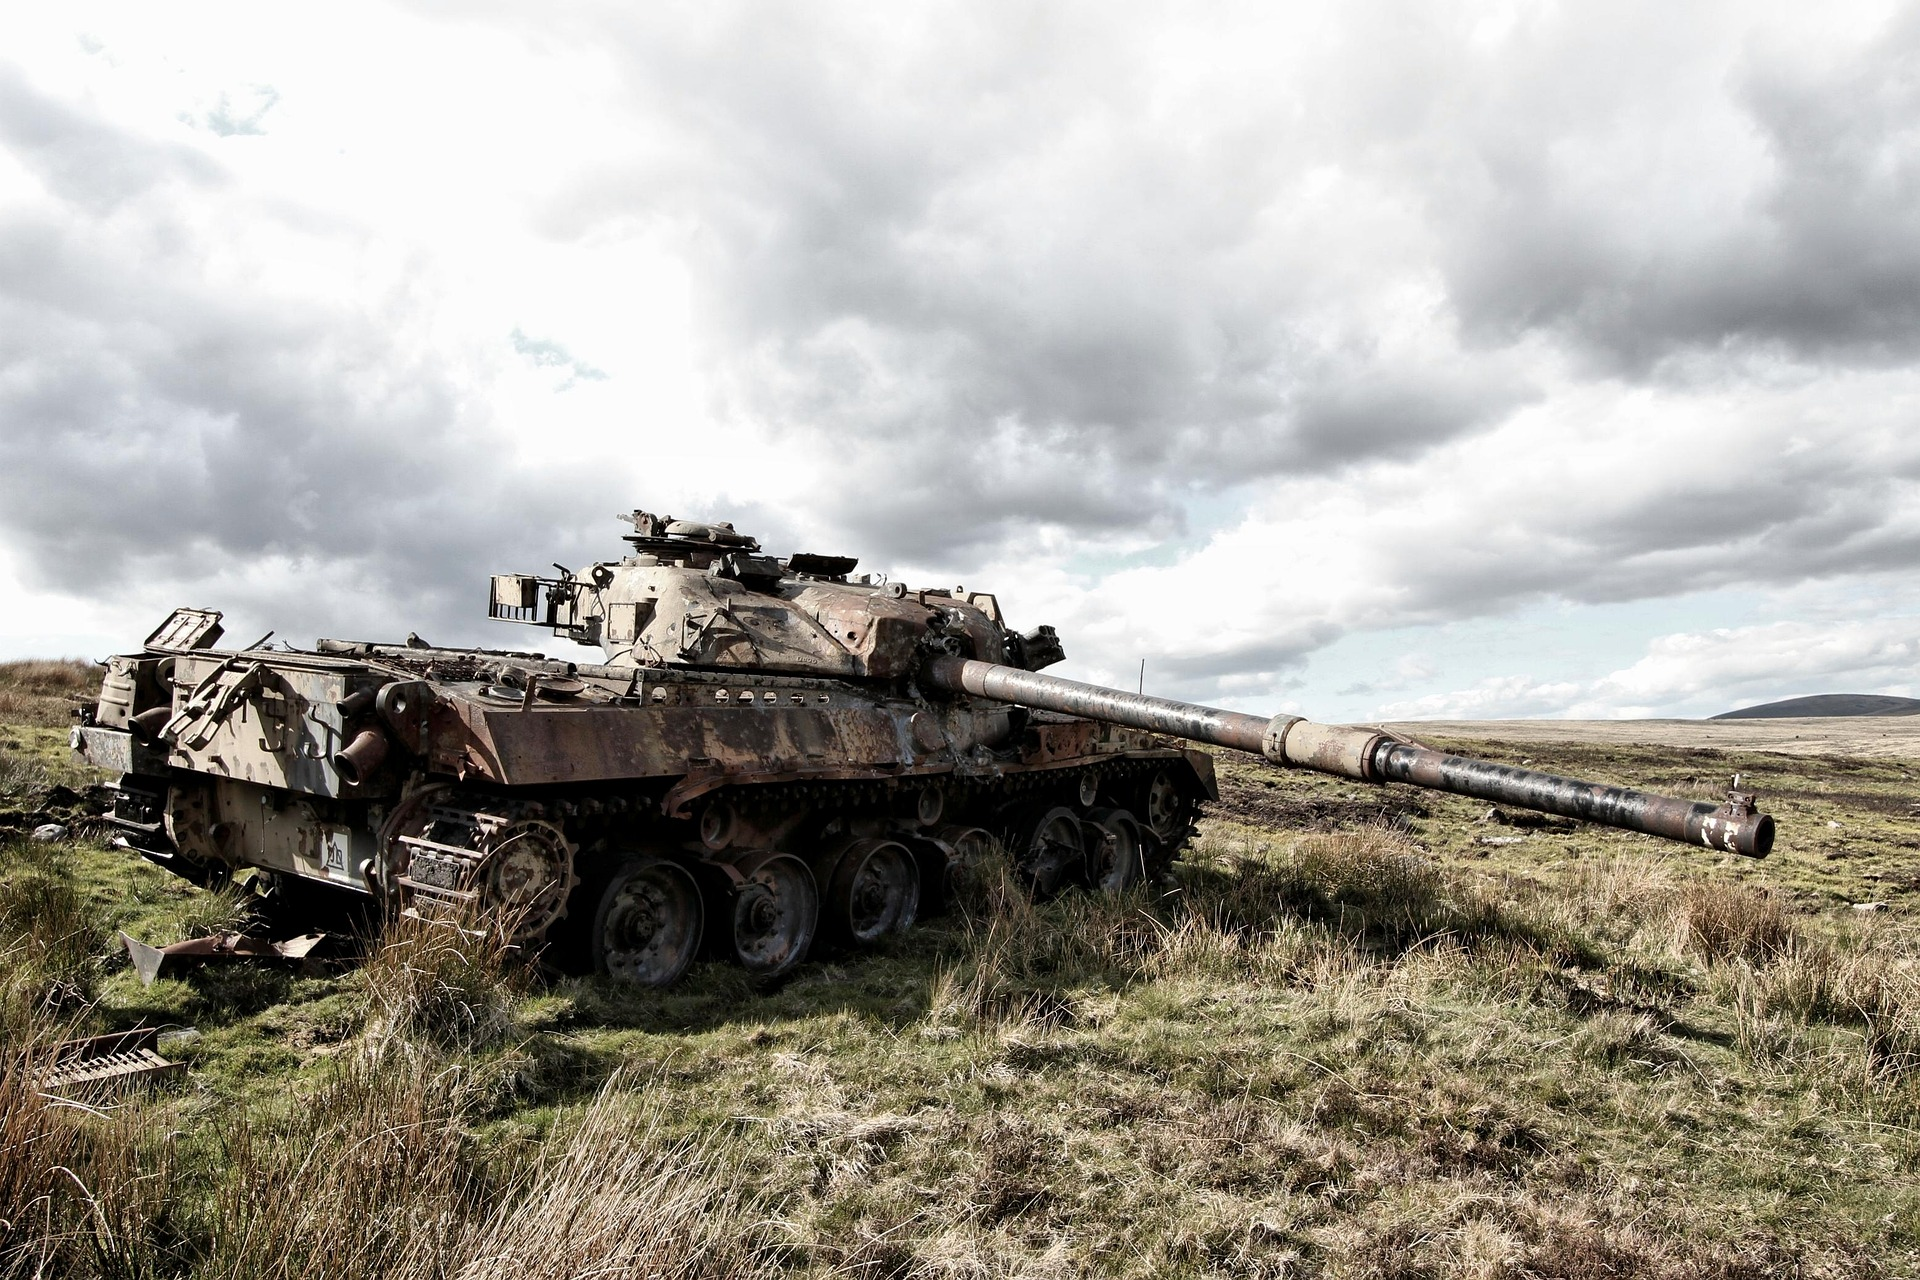
\includegraphics[width=0.45\textwidth]{../../slides/01_intro/figure/tank.jpg}
            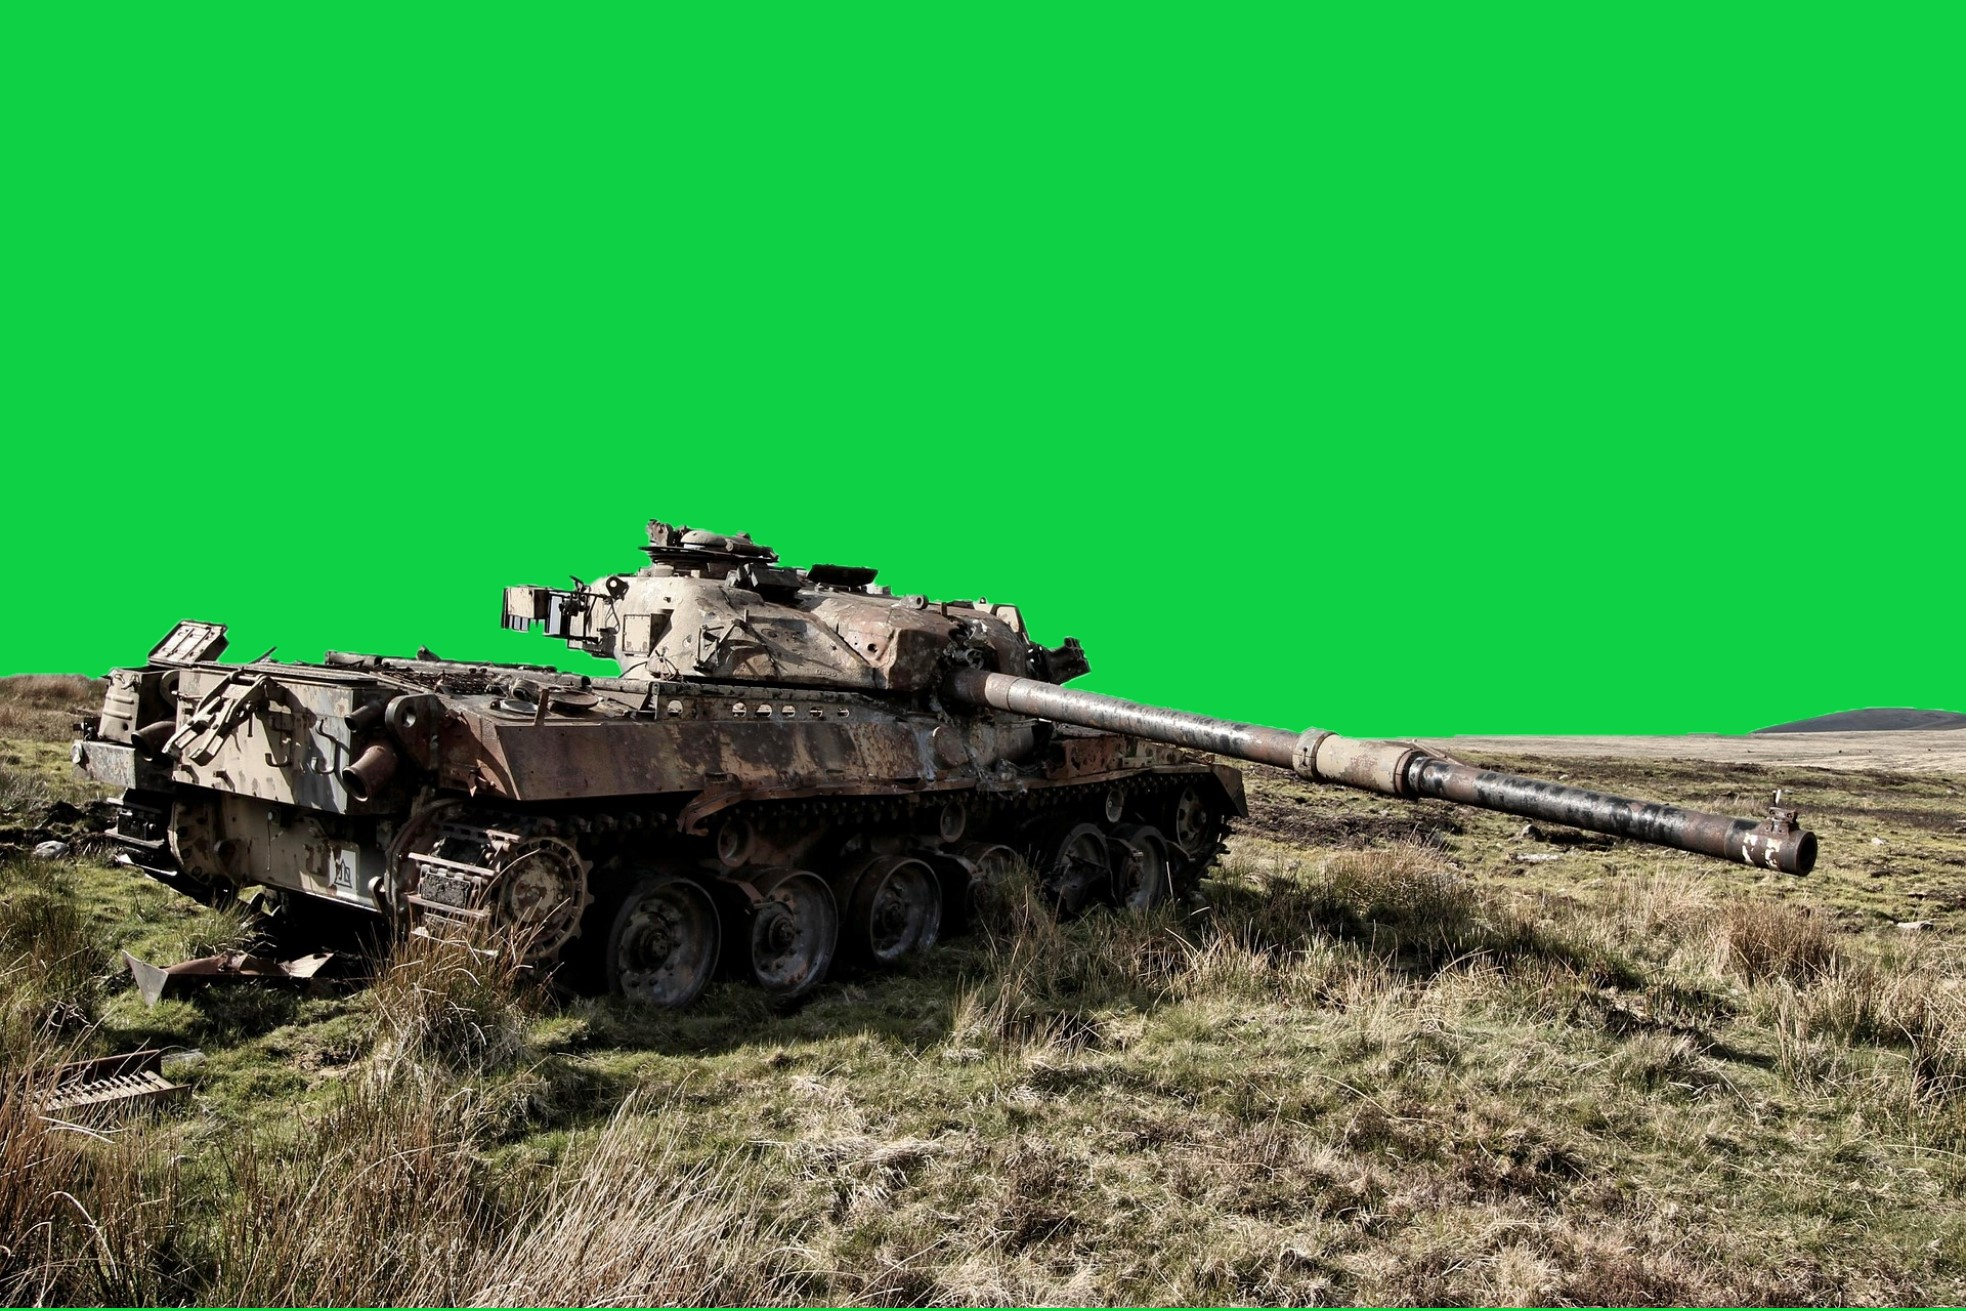
\includegraphics[width=0.45\textwidth]{../../slides/01_intro/figure/tank_green.jpg}
	        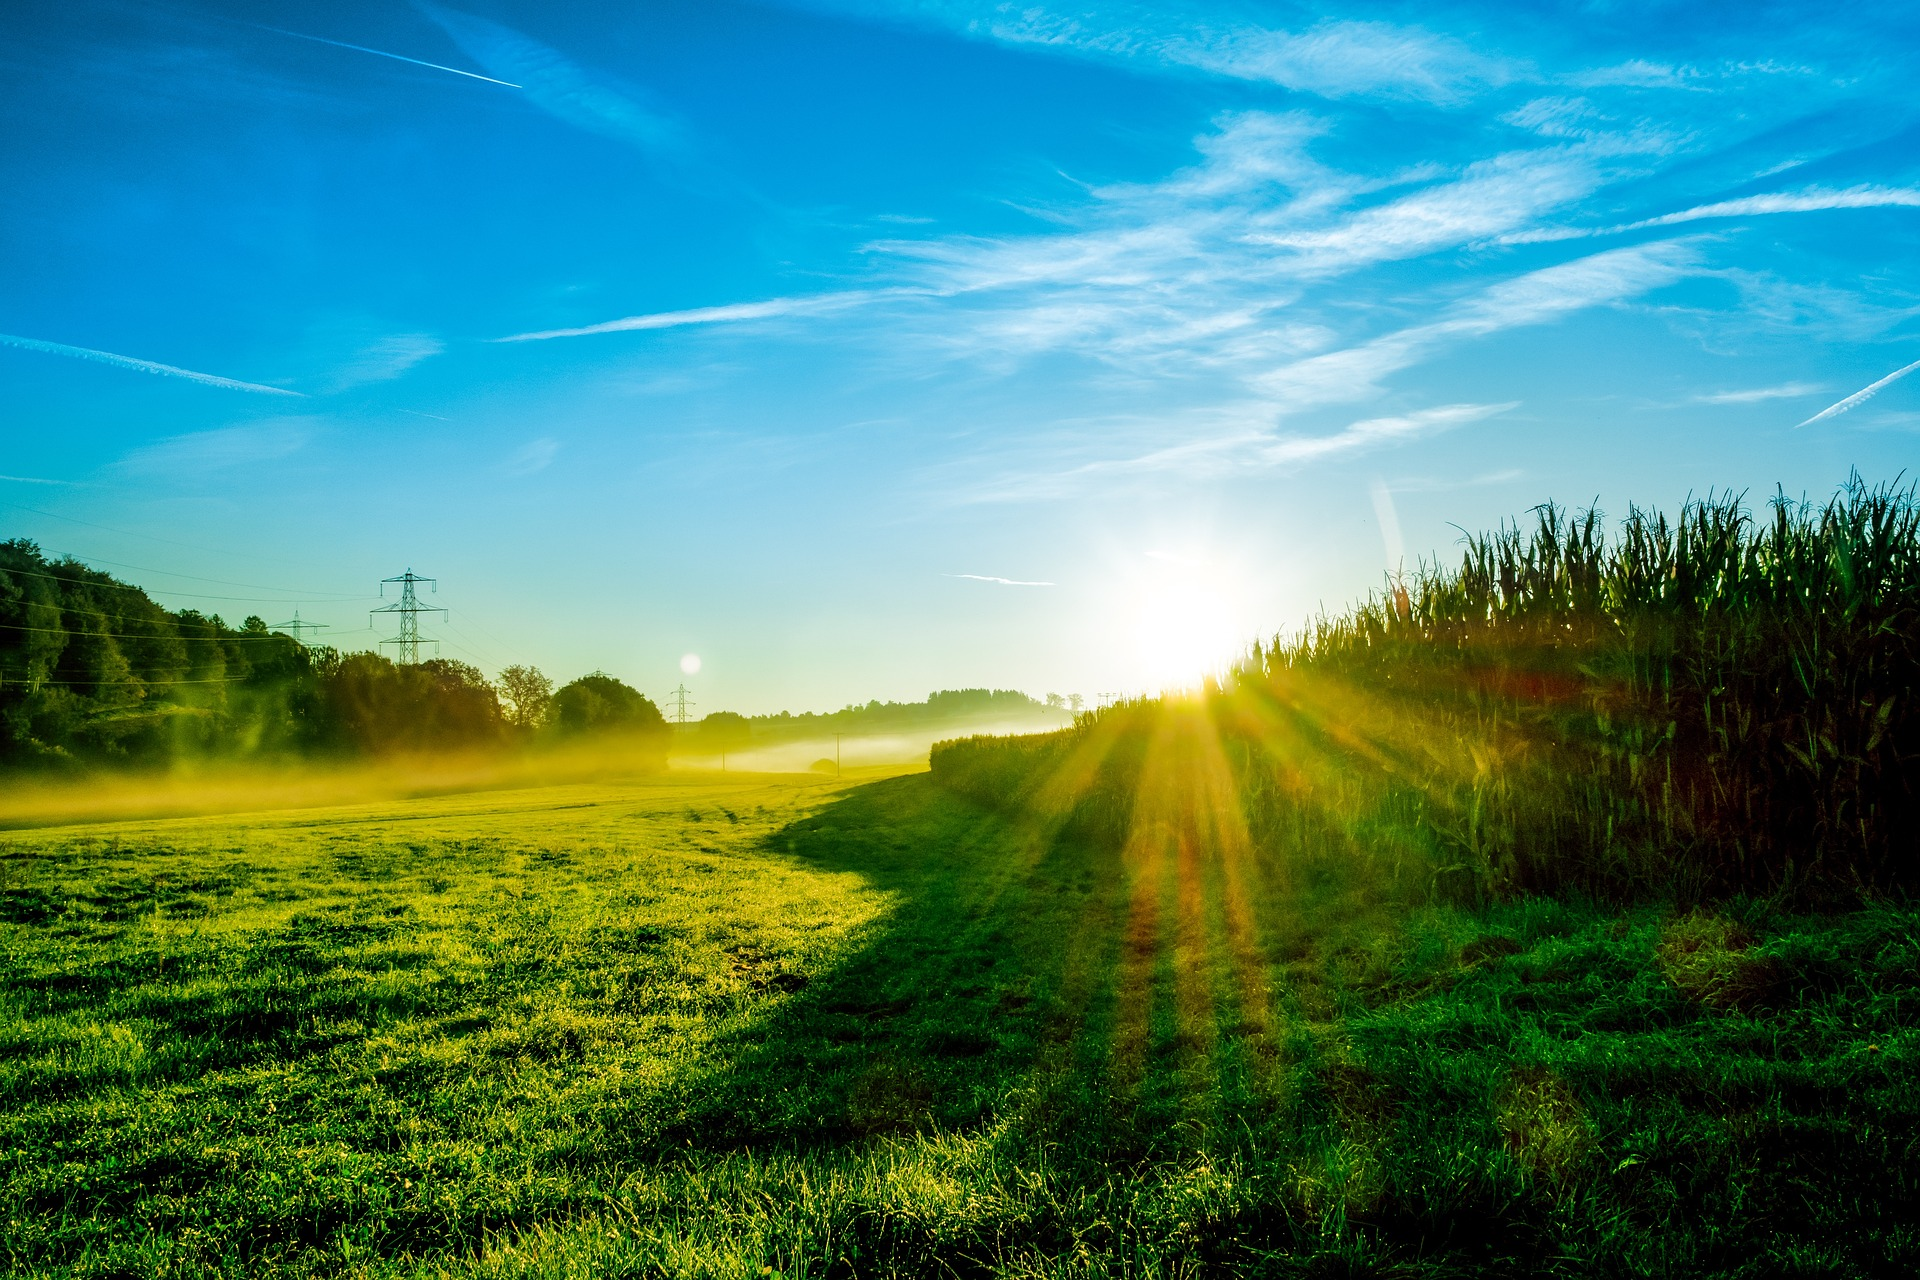
\includegraphics[width=0.45\textwidth]{../../slides/01_intro/figure/landscape.jpg}
	        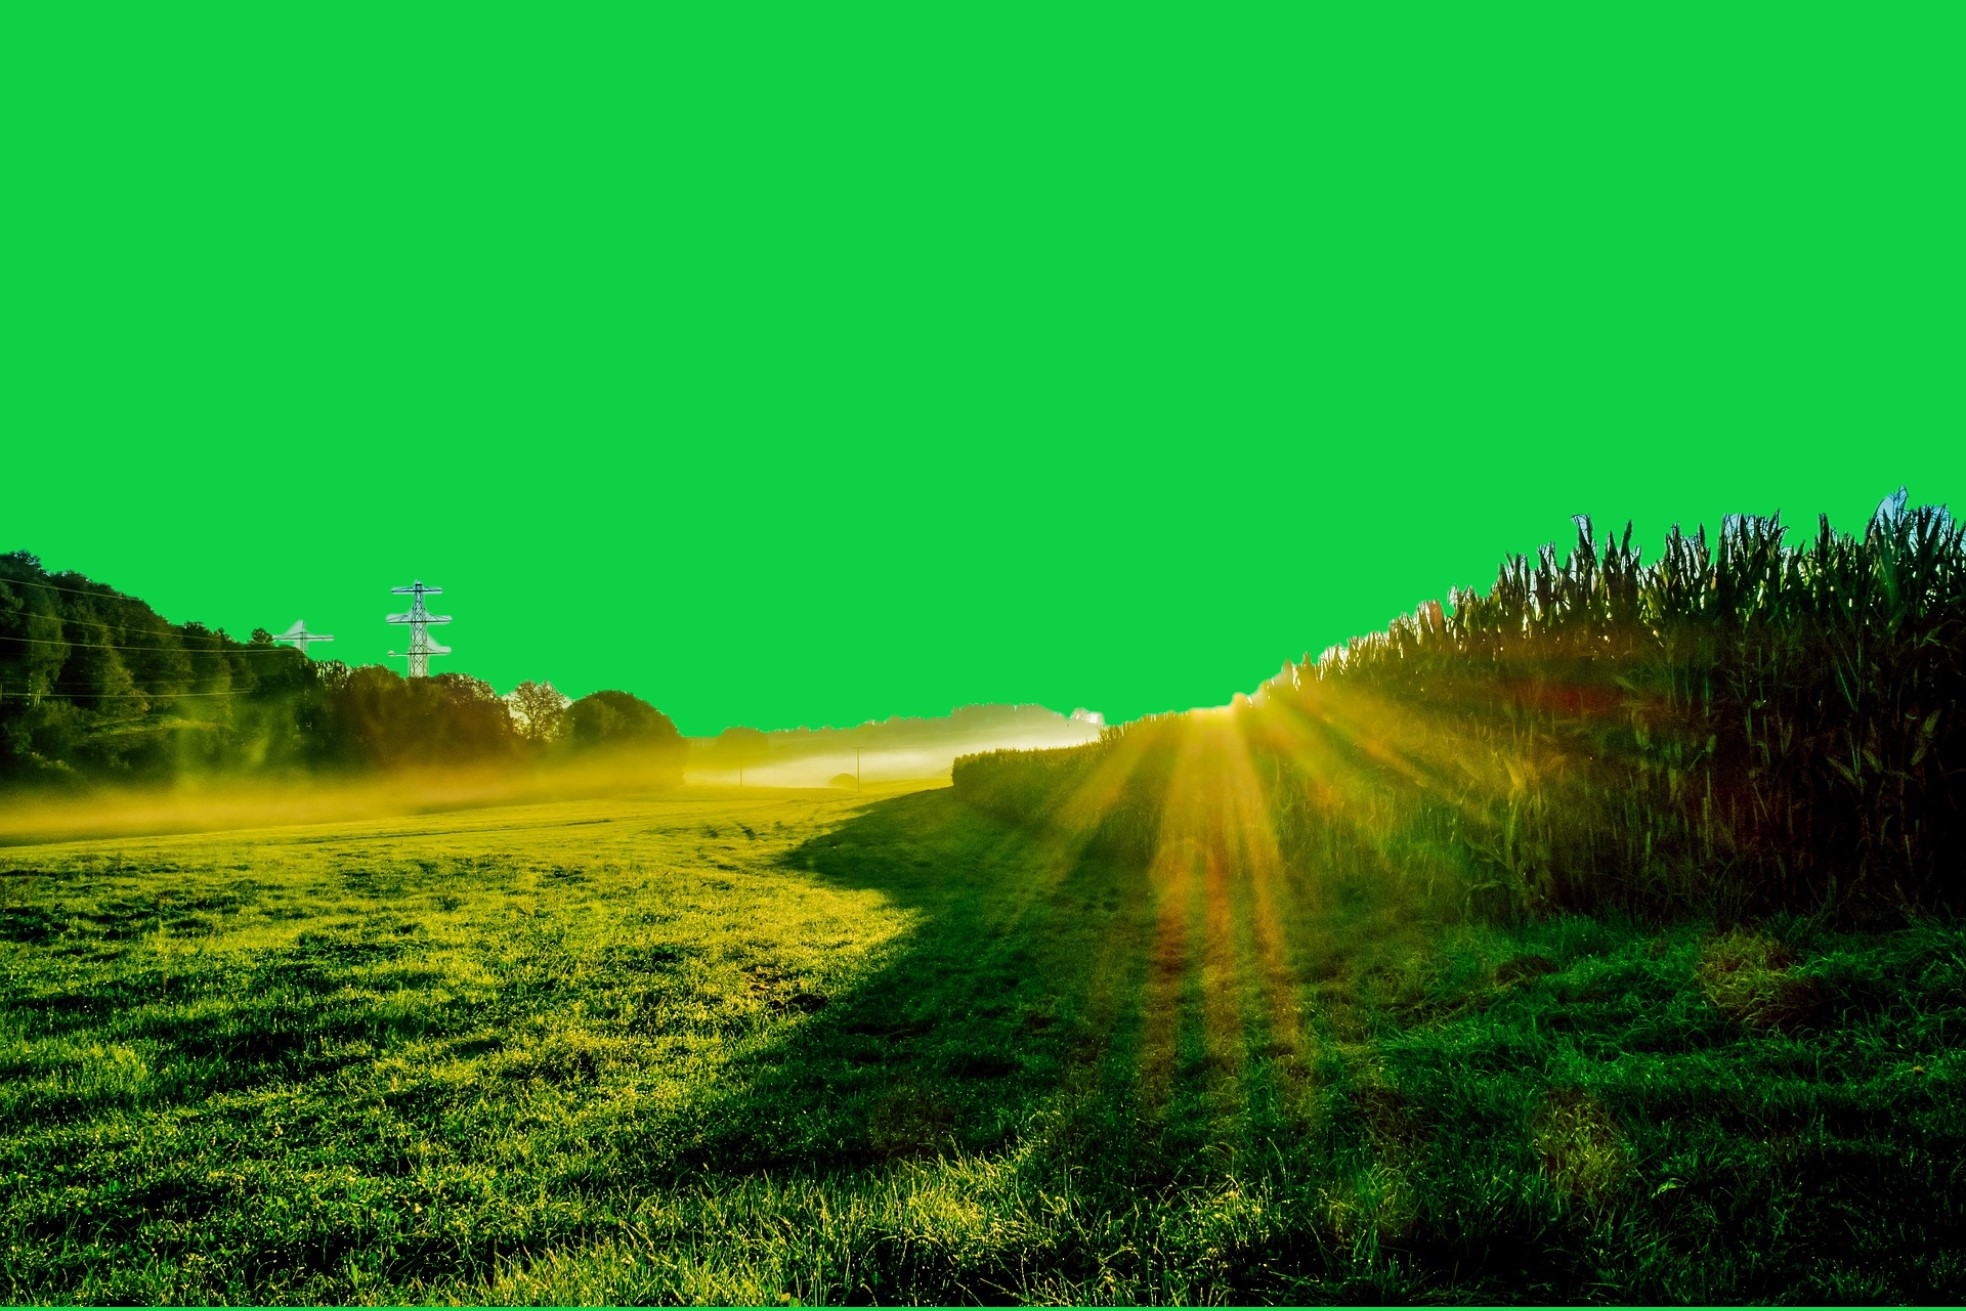
\includegraphics[width=0.45\textwidth]{../../slides/01_intro/figure/landscape_green.jpg}}
	\end{column}
	\begin{column}{0.54\textwidth}
    A cautionary tale (which never actually happened):
	\begin{itemize}
	    \item Creation of neural network to detect tanks
        \item Model shows good predictive performance in training data set
        \item Application outside training data set: failure
        \item<2-> Reasons vary depending on the source, in general: NN based its decision on irrelevant points. 
        \item<3-> E.g. model detecting weather situations: Tanks always photographed under cloudy skies; photos without tanks always taken in sunny weather.
	\end{itemize}

	\end{column}
	\end{columns}

\end{frame}

% \begin{frame}{Improve model, debug and audit}
% $\leadsto$ Insights help to identify flaws (in data or model), which can be corrected \\
% \vspace{0.9cm}
% 	\centering
%     Comment on tank example: \\
%     \medskip
%     \begin{quote}
%         ''We made exactly the same mistake in one of my projects on insect recognition. We photographed 54 classes of insects. Specimens had been collected, identified, and placed in vials. Vials were placed in boxes sorted by class. I hired student workers to photograph the specimens. Naturally they did this one box at a time; hence, one class at a time. Photos were taken in alcohol. Bubbles would form in the alcohol. Different bubbles on different days. The learned classifier was surprisingly good. But a saliency map revealed that it was reading the bubble patterns and ignoring the specimens. I was so embarrassed that I had made the oldest mistake in the book (even if it was apocryphal). Unbelievable. Lesson: always randomize even if you don’t know what you are controlling for!''
%     \end{quote}
%     \citebutton{Thomas G. Dietterich}{https://nitter.moomoo.me/tdietterich/status/1154839042623594496}
%  \end{frame}

% \begin{frame}[c]{Debug and Audit}
%     \begin{itemize}
%         %\item etwas mehr die "technische" perspektive bringen und ein paar zeilen hintergrund was debuggiung ist, warum es schon immer schwierrig war und mit ML die hölle wird. ein porgramm schreibt ein program
%         \item At first instance nearly all computer programs (CPs) have bugs
%         \begin{itemize}
%             \item[$\leadsto$] Minimizing bugs in CPs and systems is mandatory
%         \end{itemize}
%         \item Process with multiple steps to locate, understand and solve a problem
%         \begin{itemize}
%             \item[$\leadsto$] Classical debugging
%         \end{itemize}
%         \item \textbf{In ML} we have a program (CP1) writing another program (CP2)
%         \item Code of CP2 (the ML model) is not readable $\leadsto$ How to debug the model?
%         \begin{itemize}
%             \item[$\leadsto$] Investigate the data
%             \item[$\leadsto$] Simplify as far as possible
%             \item[$\leadsto$] Verify the mathematics
%             \item[$\leadsto$] Make the code more complex step by step
%         \end{itemize}
%     \end{itemize}
% \end{frame}

% \begin{frame}{Clever Hans \citebutton{Lapuschkin et al. 2019}{https://www.nature.com/articles/s41467-019-08987-4}}

% 	\centering
% 	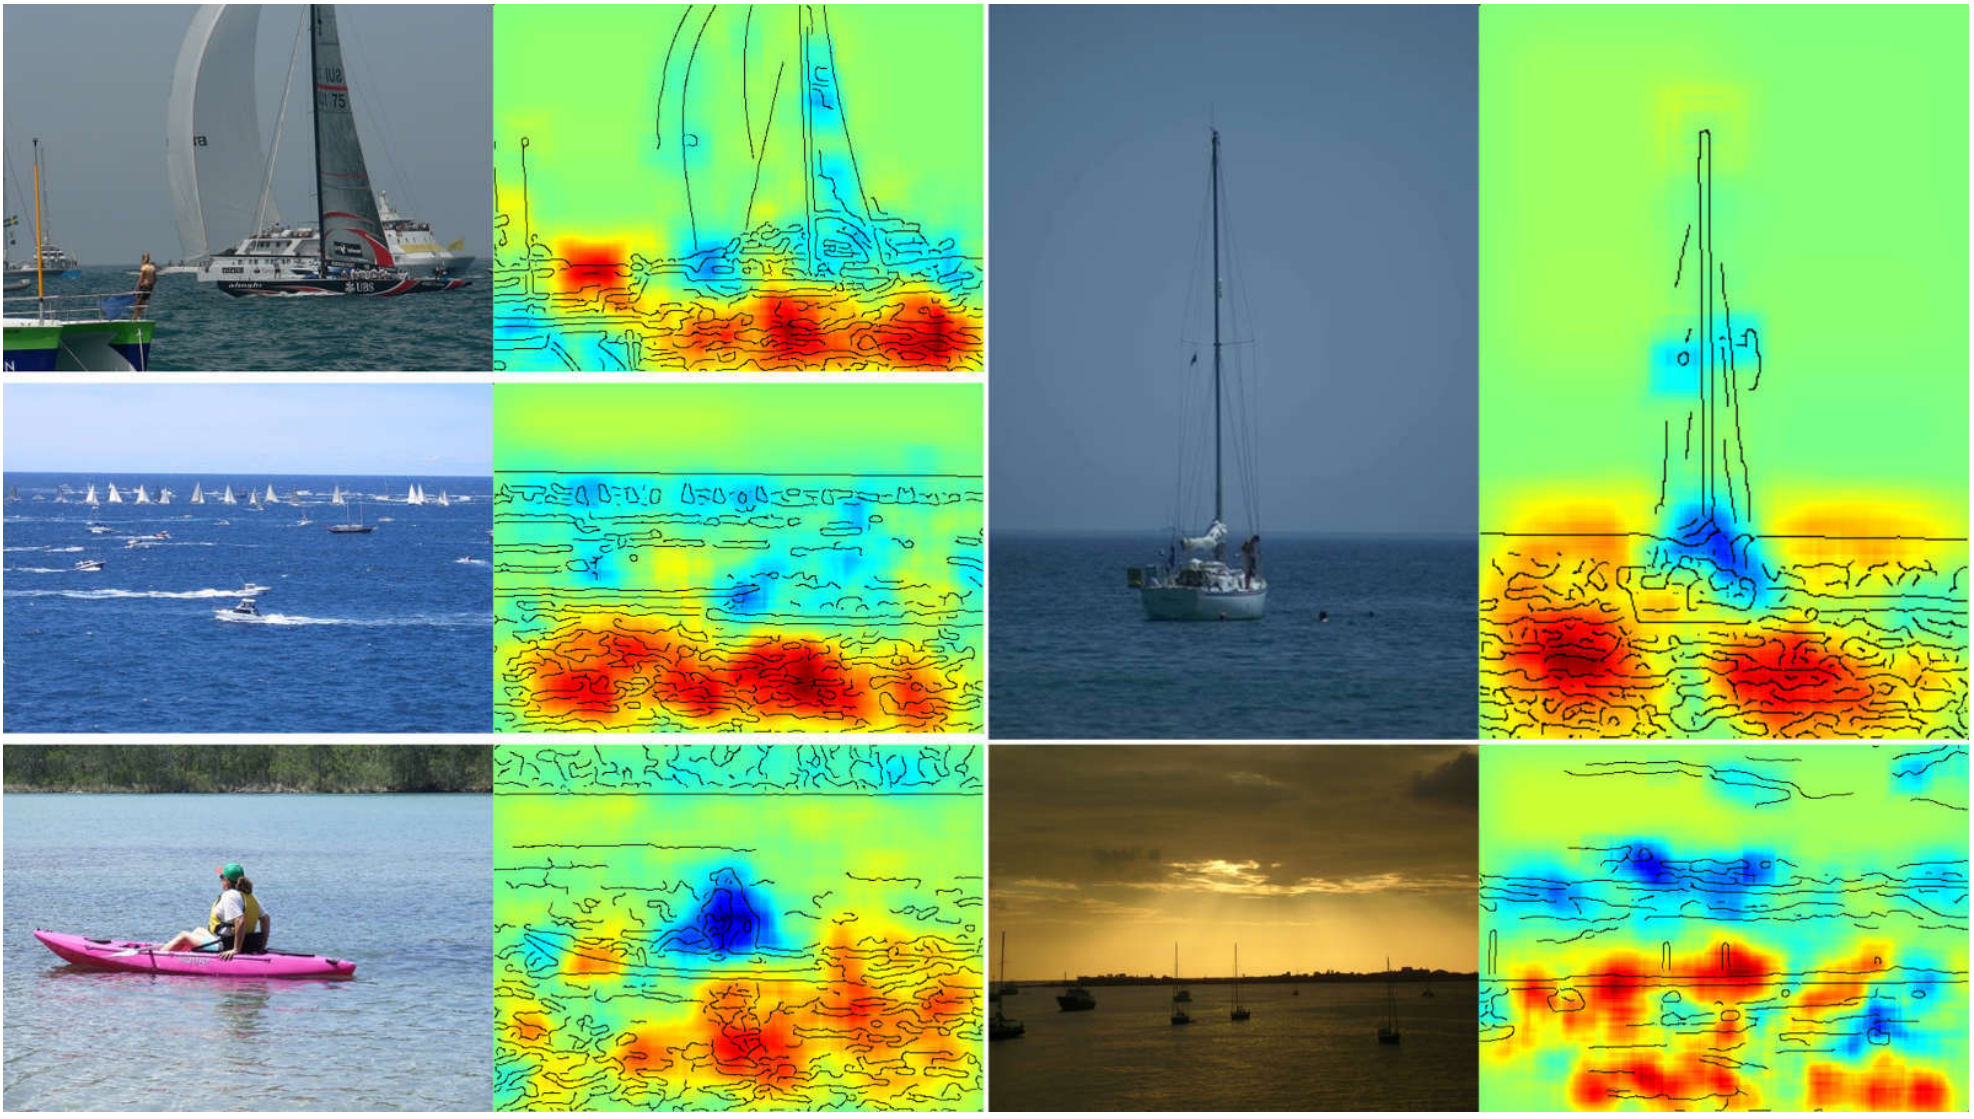
\includegraphics[width=0.6\textwidth]{figure/boats_maps.PNG}

% \end{frame}

\begin{frame}{Understand and control individual predictions}
    $\leadsto$ Explaining individual decisions can prevent unwanted actions based on the model \\
    \medskip
    \textbf{Example:} Credit Risk Application. $\textbf{x}$: customer and credit information; $y$: grant or reject credit
	
	\only<1>{\begin{center}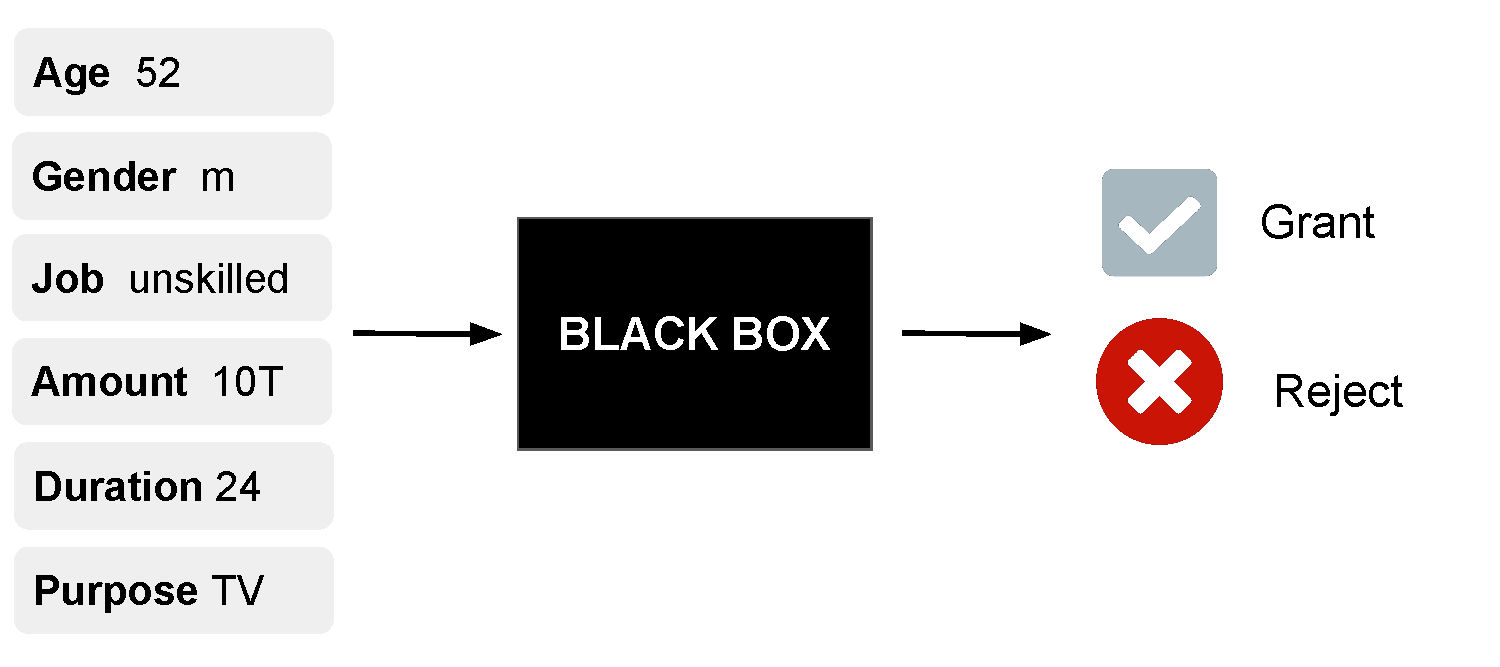
\includegraphics[width=0.6\linewidth, page=1]{../../slides/01_intro/figure/counterfactuals_credit.pdf} \end{center}

	Questions:}
	\begin{itemize}
		\item Why was the credit rejected?
		\item Is it a fair decision?
		\item \textbf{How should $\xv$ be changed so that the credit is accepted?}
	\end{itemize}
	
	%Counterfactual Explanations provide answers in the form of "What-If"-scenarios.
	%\only<2>{\begin{center}\includegraphics[width=0.6\linewidth, page=2]{../../slides/01_intro/figure/counterfactuals_credit.pdf} \end{center}

	%``If the person was more skilled and the credit amount had been reduced to \$8.000,\\ the credit would have been granted."} 
\end{frame}

%%%

\begin{frame}{Justification and fairness}
    $\leadsto$ Investigate if and why biased, unexpected or discriminatory predictions were made \\
    \bigskip
    \textbf{Example:} COMPAS
    \smallskip
    \begin{itemize}
        \item Correctional Offender Management Profiling for Alternative Sanctions (COMPAS)
        \smallskip
        \item Commercial algorithm used by judges to assess defendant’s likelihood of re-offending
        %\pause
        \smallskip
        \item Predict recidivism risk
        \begin{itemize}
            \item i.e., criminal re-offense after previous crime, resulting in jail booking
            \smallskip
            \item different risk levels: high risk, medium risk or low risk
        \end{itemize}
        %\pause
        \smallskip
        \item Evaluation of recidivism risk based on a questionnaire the defendant has to answer
    \end{itemize}

\end{frame}

\begin{frame}{Justification and fairness: COMPAS~\citebutton{Larson et al. 2016}{https://www.propublica.org/article/how-we-analyzed-the-compas-recidivism-algorithm}}
    $\leadsto$ Investigate if and why biased, unexpected or discriminatory predictions were made \\
    \medskip
    Descriptive data analysis: 
    
    \centering
    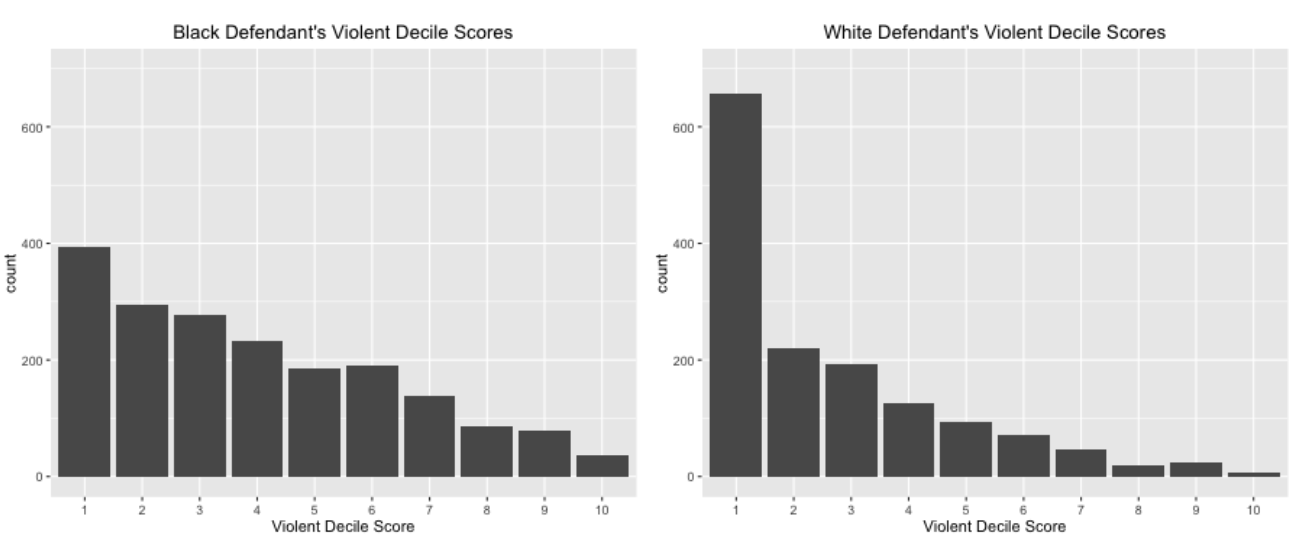
\includegraphics[width=0.7\textwidth]{../../slides/01_intro/figure/compass_black_white.PNG}
    % source https://www.propublica.org/article/how-we-analyzed-the-compas-recidivism-algorithm

    Decile score: 1 (low risk) to 10 (high risk)

	$\leadsto$ Model skewed towards low risk for white defendants
	
	$\leadsto$ Strong indication that the model is discriminating black defendants
	
	$\leadsto$ Use IML to investigate if and how much the model uses the defendants' origin.
\end{frame}

% \begin{frame}{Justification and fairness: COMPAS~\citebutton{Alvarez-Melis and Jaakkola 2018}{https://arxiv.org/pdf/1806.08049.pdf}}
%     $\leadsto$ Investigate if and why biased, unexpected or discriminatory predictions were made \\
%     \medskip
%     The underlying classifier is a logistic regression. Feature effects analysis for two exemplary defendants, using different interpretation methods (SHAP and LIME): \\
%     $\leadsto$ The methods give for every feature a number mirroring the impact on violence score. 
%     \vspace{0.5cm}
    
%     \centering
%     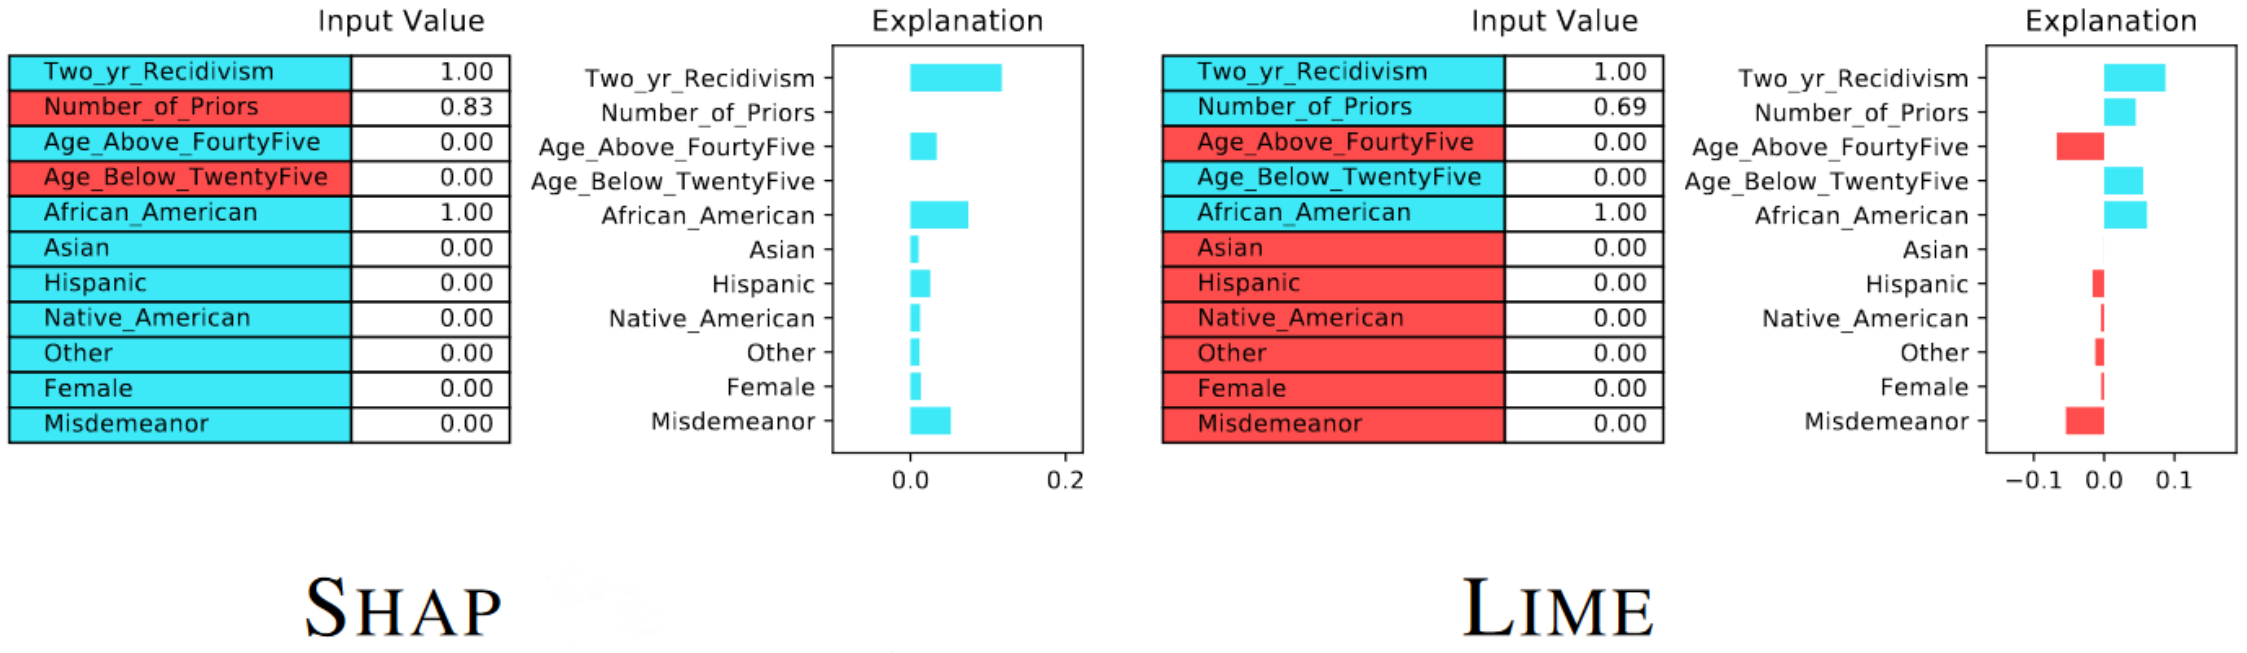
\includegraphics[width=0.95\textwidth]{../../slides/01_intro/figure/COMPAS_shap_lime_example.png}
    
%     \vspace{0.2cm}
%     $\leadsto$ In both cases the race (african american) has a noticeable positive impact on violent score
% \end{frame}





% \begin{frame}{Motivation - Adversarial Examples \citebutton{Goodfellow et al. 2016}{https://arxiv.org/pdf/1412.6572.pdf}}

%     \begin{center}
%     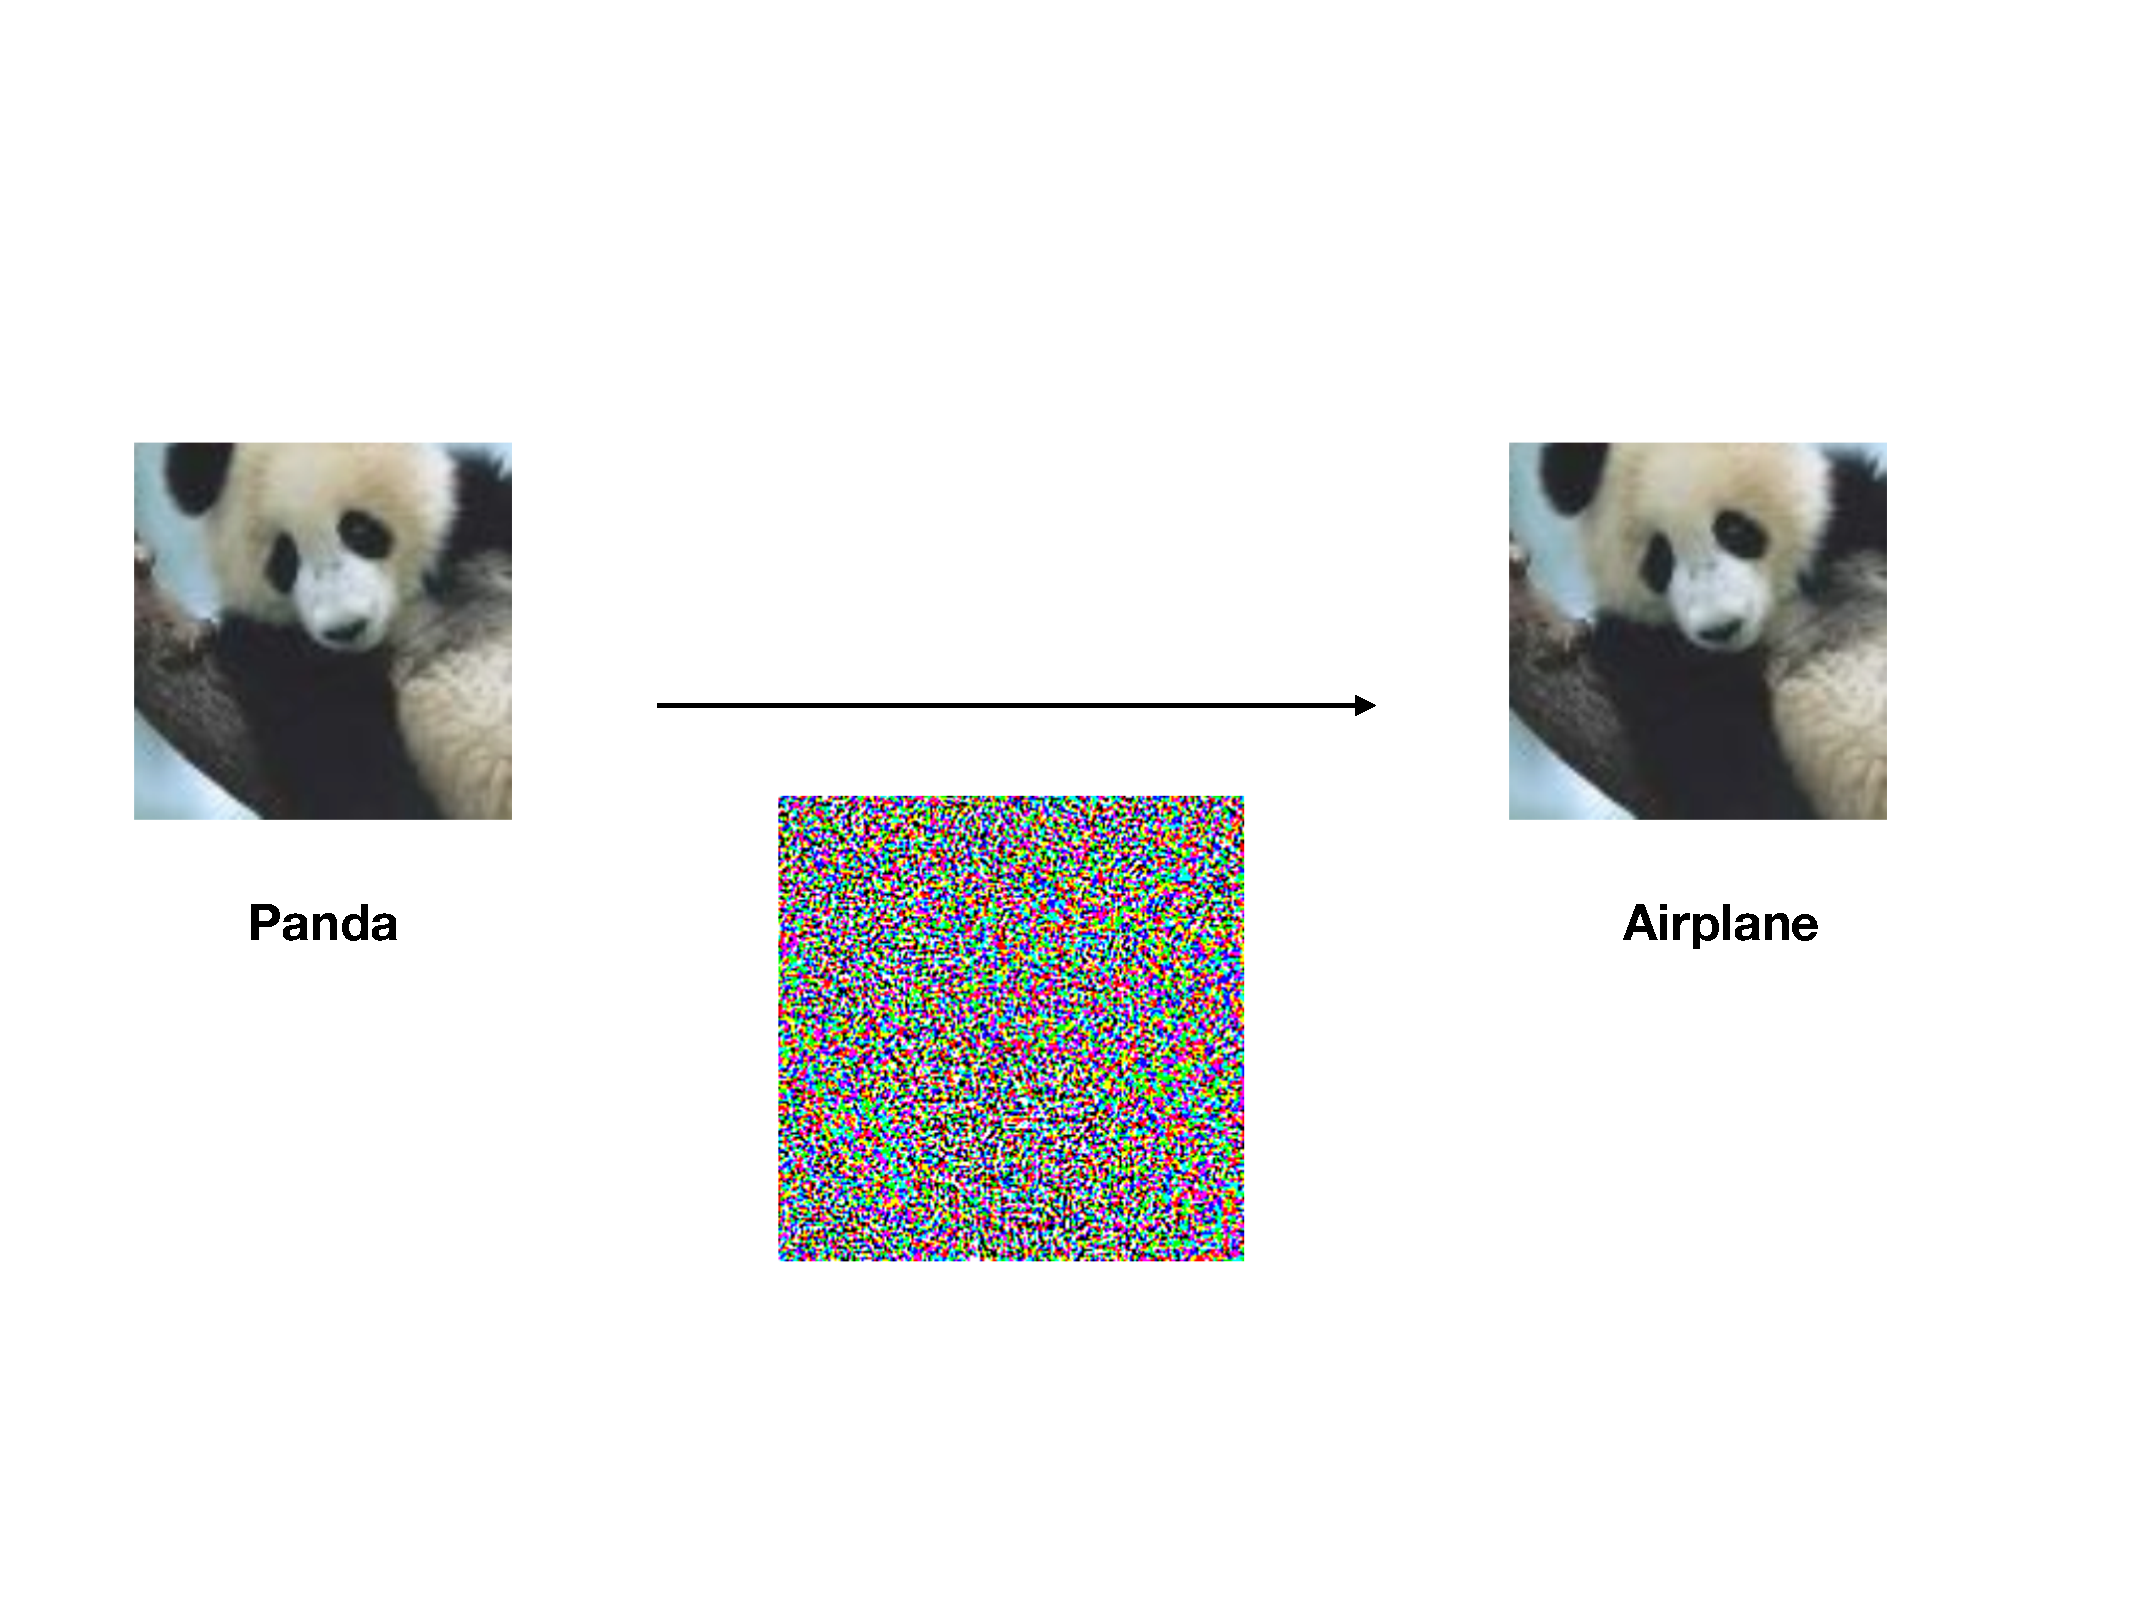
\includegraphics[width=0.7\textwidth]{figure/panda-airplane.pdf}
%     \end{center}
% 	\bigskip

% 	$\rightarrow$ ML Models might not capture human-like understanding
% \end{frame}


% \begin{frame}{Adversarial Noise \citebutton{Goodfellow et al. 2016}{https://arxiv.org/pdf/1412.6572.pdf}}
%     \begin{center}
%     \includegraphics[width=0.65\textwidth]{figure/adv-noise.pdf}
%     % https://arxiv.org/pdf/1412.6572.pdf
% 	\end{center}
% 	\normalsize
% 	%\bigskip
% 	$\rightarrow$\textbf{Adversarial Noise:} Noise not visible to \textbf{humans} but results in incorrect classification results
% \end{frame}

% \begin{frame}[c]{Adversarial Examples~\citebutton{Goodfellow et al. 2016}{https://arxiv.org/pdf/1412.6572.pdf}}
    
%     \centering
%     \includegraphics[width=0.7\textwidth]{figure/adv-noise-2.pdf}
	
% \end{frame}

% \begin{frame}{Performance vs. Interpretability}
%     \centering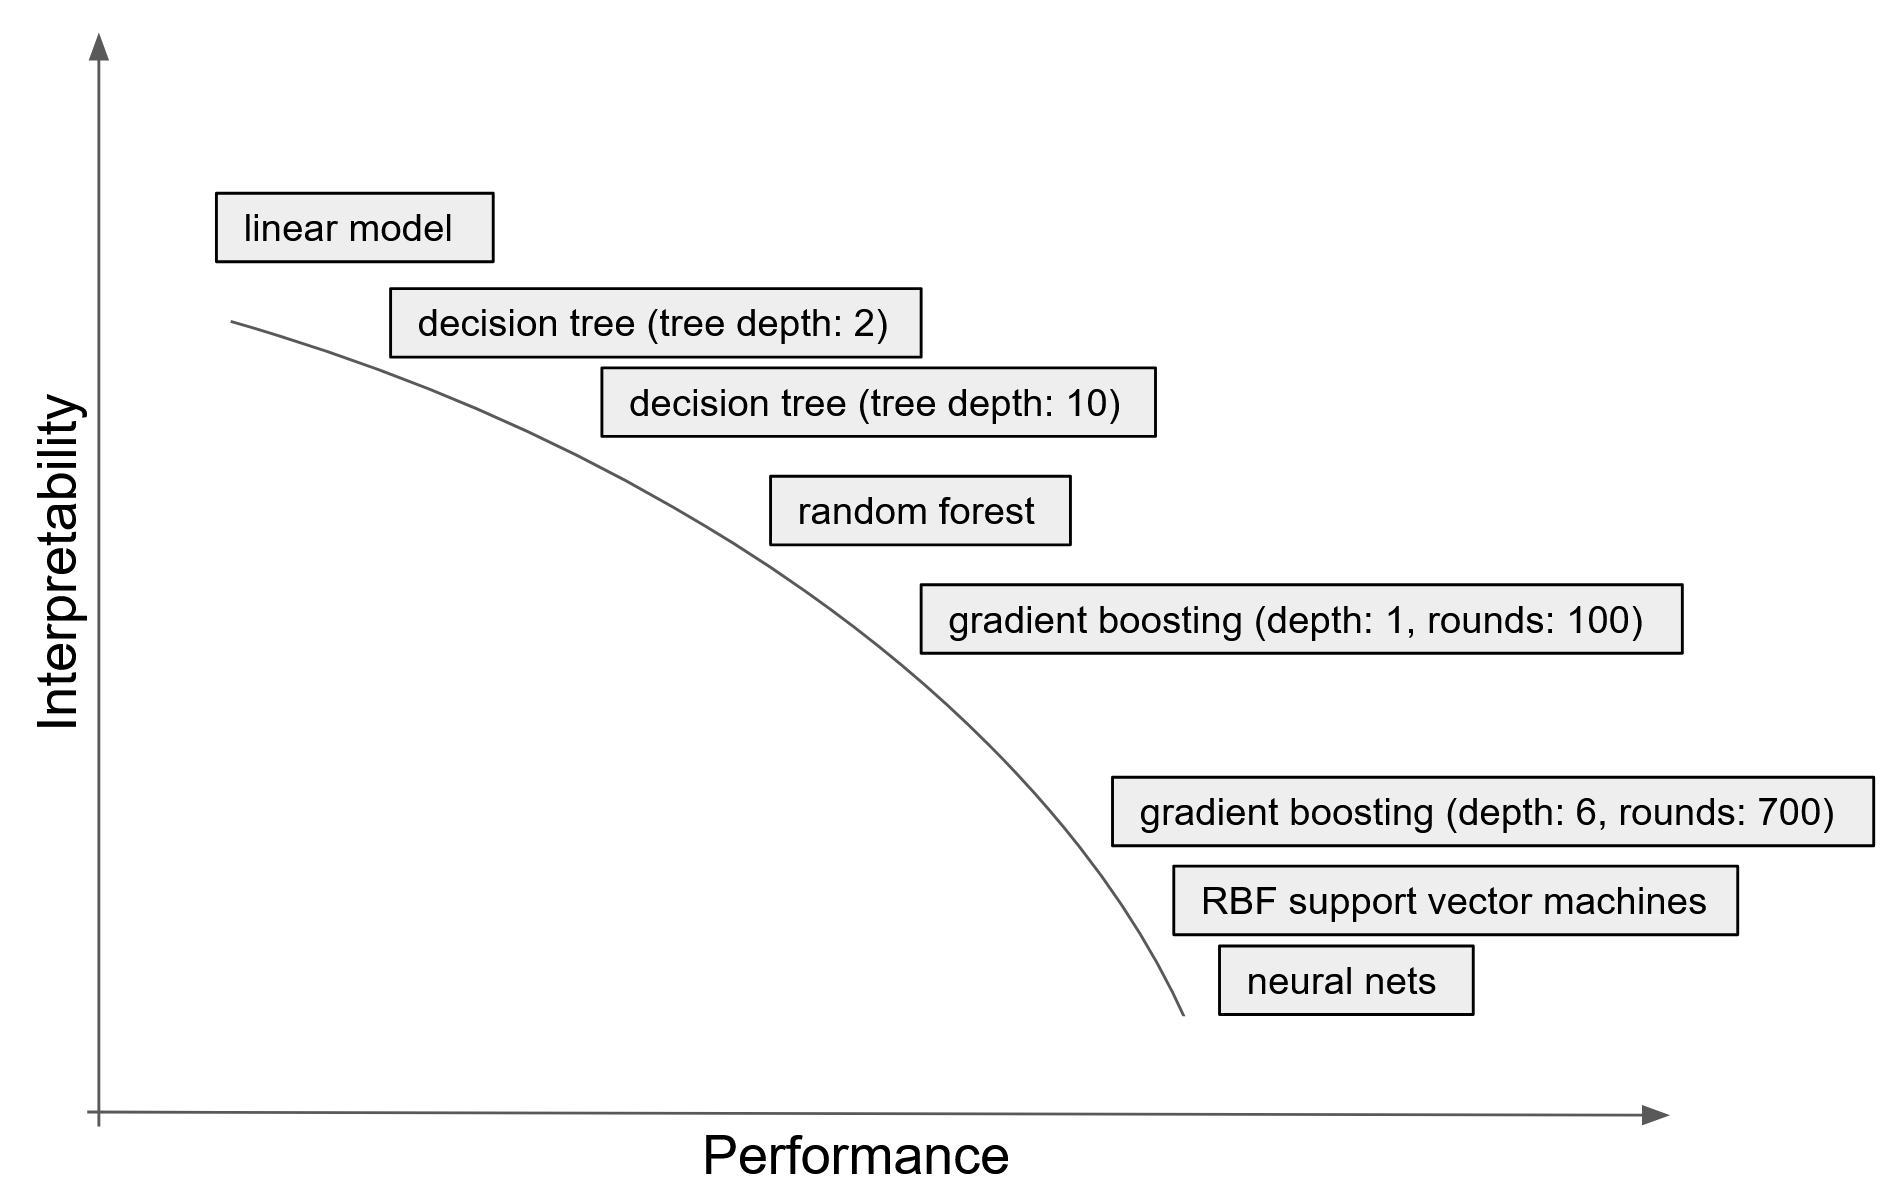
\includegraphics[width=0.7\textwidth]{../../slides/01_intro/figure/performance_vs_interpretability.png}
%     % Quelle: https://docs.google.com/presentation/d/12ZPrTjBKEUT-7drdyUJCQGK0oHVDtYIVd2_6byE62f0/edit?usp=sharing
%     %\centering \citebutton{Scott Fortmann-Roe (2012)}{http://scott.fortmann-roe.com/docs/BiasVariance.html}
% \end{frame}


\begin{frame}{Intrinsic vs. Model-Agnostic}
%	\begin{center}
%		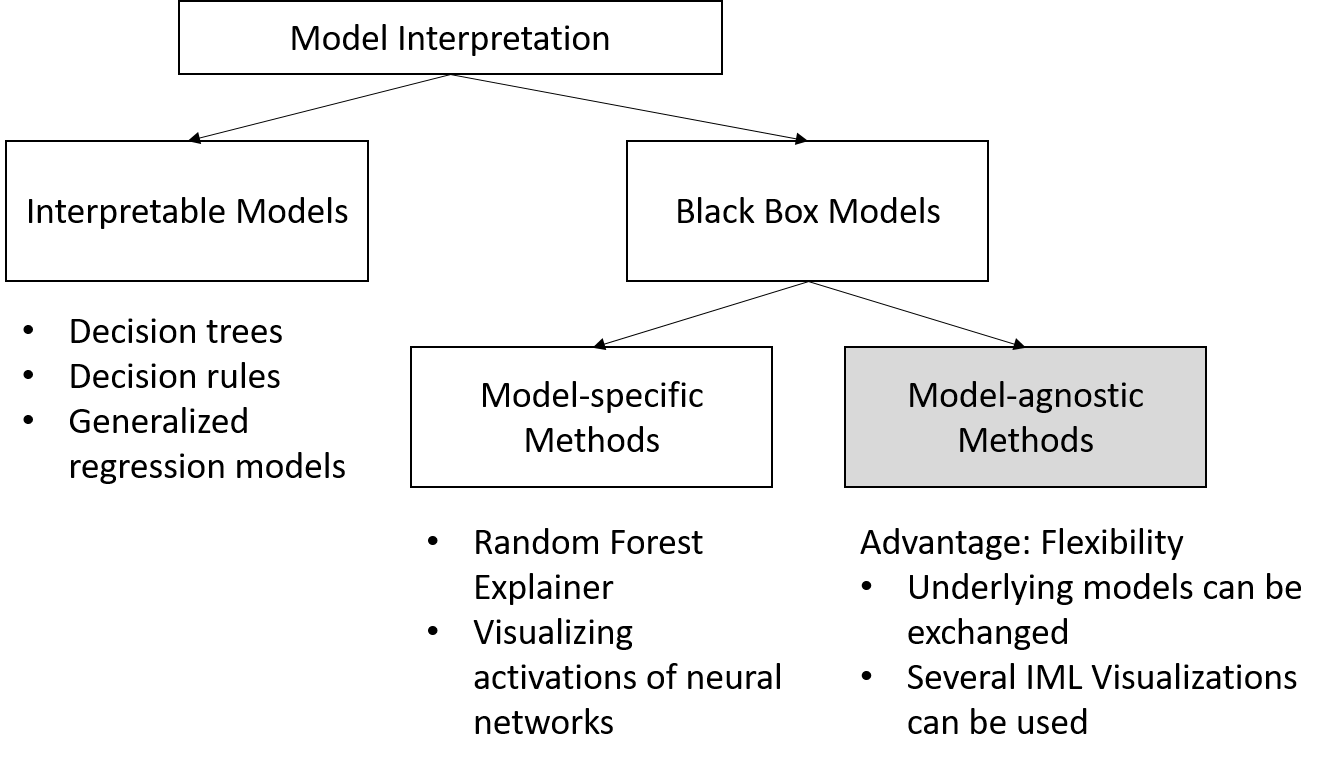
\includegraphics[width=0.8\textwidth]{figure/overview}
%	\end{center}
	\begin{center}
	    
		\begin{tikzpicture}[every path/.style={->,line width=0.35mm,thick},
                        every label/.append style={align=left, font=\footnotesize, text width=4cm}]
        \node[main node] (1) { Model Interpretation };
        \node[main node,
            label={below: 
            \tab[0.25cm] - Decision trees \\ 
            \tab[0.25cm] - Decision rules \\ 
            \tab[0.25cm] - GLMs}
            ] (2) [below left = 1cm and 0cm of 1]  { Interpretable Models };
        \node[main node] (3) [below right = 1cm and -0cm of 1] { Black Box Models };
        \node[main node,
            label={below: 
            - Random forest explainer \\ - Visualizing activations of neural networks}
            ] (4) [below left = 1cm and -1cm of 3] { Model-specific Methods  };
        \node[main node, fill=lightgray,
            label={below:
            - \textbf{Advantage:} Applicable to any model\\ 
            - Feature effect methods\\
            - Feature importance methods}
            ] (5) [below right = 1cm and -1cm of 3] { Model-agnostic Methods };
        \draw (1) -- (2);
        \draw (1) -- (3);
        \draw (3) -- (4);
        \draw (3) -- (5);

    \end{tikzpicture}
	\end{center}
\end{frame}


% \begin{frame}{Intrinsic vs. Model-Agnostic}
% 		\begin{columns}
% 		\begin{column}{0.75\textwidth}
% 	\begin{itemize}
% 		\item<1-> Intrinsically interpretable models:
% 		\medskip
		
% 		\begin{itemize}
% 		%\itemsep1em
% 			\item Examples: linear model and decision tree
% 			\item Interpretable because of simple model structure, \\
% 			e.g., weighted combination of feature values or tree structure
% 			\item Difficult to interpret with many features / complex interactions
% 		\end{itemize}
		
% 	\medskip
% 	%\pause
% 		\item<2-> Model-agnostic interpretation methods:
% 		\medskip
% 		\begin{itemize}
% 		%\itemsep1em
% 			\item Applied after training (post-hoc)
% 			\item Work for any model $\leadsto$ only access to data and model required
% 			%\item Also work for more complex black box models
% 			\item Can also be applied to intrinsically interpretable models,\\ e.g., feature importance for linear model %decision trees
% 			\item Different types of explanations:\\
% 			feature or data attribution, counterfactual explanations
% 		\end{itemize}
% 	\end{itemize}
% 	\end{column}
% 	\begin{column}{0.25\textwidth}
		
%   \only<1-2>{\begin{tikzpicture}[scale=0.75, transform shape]
%   \usetikzlibrary{arrows}
%     \usetikzlibrary{shapes}
%      \tikzset{treenode/.style={draw, circle, font=\small}}
%      \tikzset{line/.style={draw, thick}}
%      \node [treenode, draw=red] (a0) {$a_0$};
%      \node [treenode, below=0.75cm of a0, xshift=-1cm]  (a1) {$a_1$};
%      \node [treenode, draw=red, below=0.75cm of a0, xshift=1cm]  (a2) {$a_2$};
     
%      \node [treenode, draw=red, below=0.75cm of a2, xshift=-1cm] (a3) {$a_3$};
%      \node [treenode, below=0.75cm of a2, xshift=1cm]  (a4) {$a_4$};
     
%      \node [treenode, below=0.75cm of a3, xshift=-1cm] (a5) {$a_5$};
%      \node [treenode, below=0.75cm of a3, xshift=1cm]  (a6) {$a_6$};
     
%      \path [line] (a0.south) -- + (0,-0.4cm) -| (a1.north) node [midway, above] {$x_1<0.3$};
%      \path [line] (a0.south) -- +(0,-0.4cm) -|  (a2.north) node [midway, above] {$x_1\geq0.3$};
     
%      \path [line] (a2.south) -- + (0,-0.4cm) -| (a3.north) node [midway, above] {$x_1<0.6$};;
%      \path [line] (a2.south) -- +(0,-0.4cm) -|  (a4.north) node [midway, above] {$x_1\geq0.6$};
     
          
%      \path [line] (a3.south) -- + (0,-0.4cm) -| (a5.north) node [midway, above] {$x_2<0.2$};;
%      \path [line] (a3.south) -- +(0,-0.4cm) -|  (a6.north) node [midway, above] {$x_2\geq0.2$};
     
%   \end{tikzpicture}}
% 	\end{column}
% 	\end{columns}
% \end{frame}

% \begin{frame}{Model-Agnostic Interpretability}
% 	\begin{itemize}
% 		\itemsep1em
% 		\item Model-agnostic interpretation methods work for \textbf{any} kind of machine learning model.
% 		\item Explanation type is not tied to the underlying model type.
% 		\item Only access to data and trained model is required.\\
% 		 No further knowledge about the model itself is necessary.
% 		\item There are multiple types of explanations:\\
% 		feature attribution, data attribution, or counterfactual explanations.
% 	\end{itemize}
% \end{frame}


\begin{frame}{Types of Explanations}
% 	\begin{center}
% 		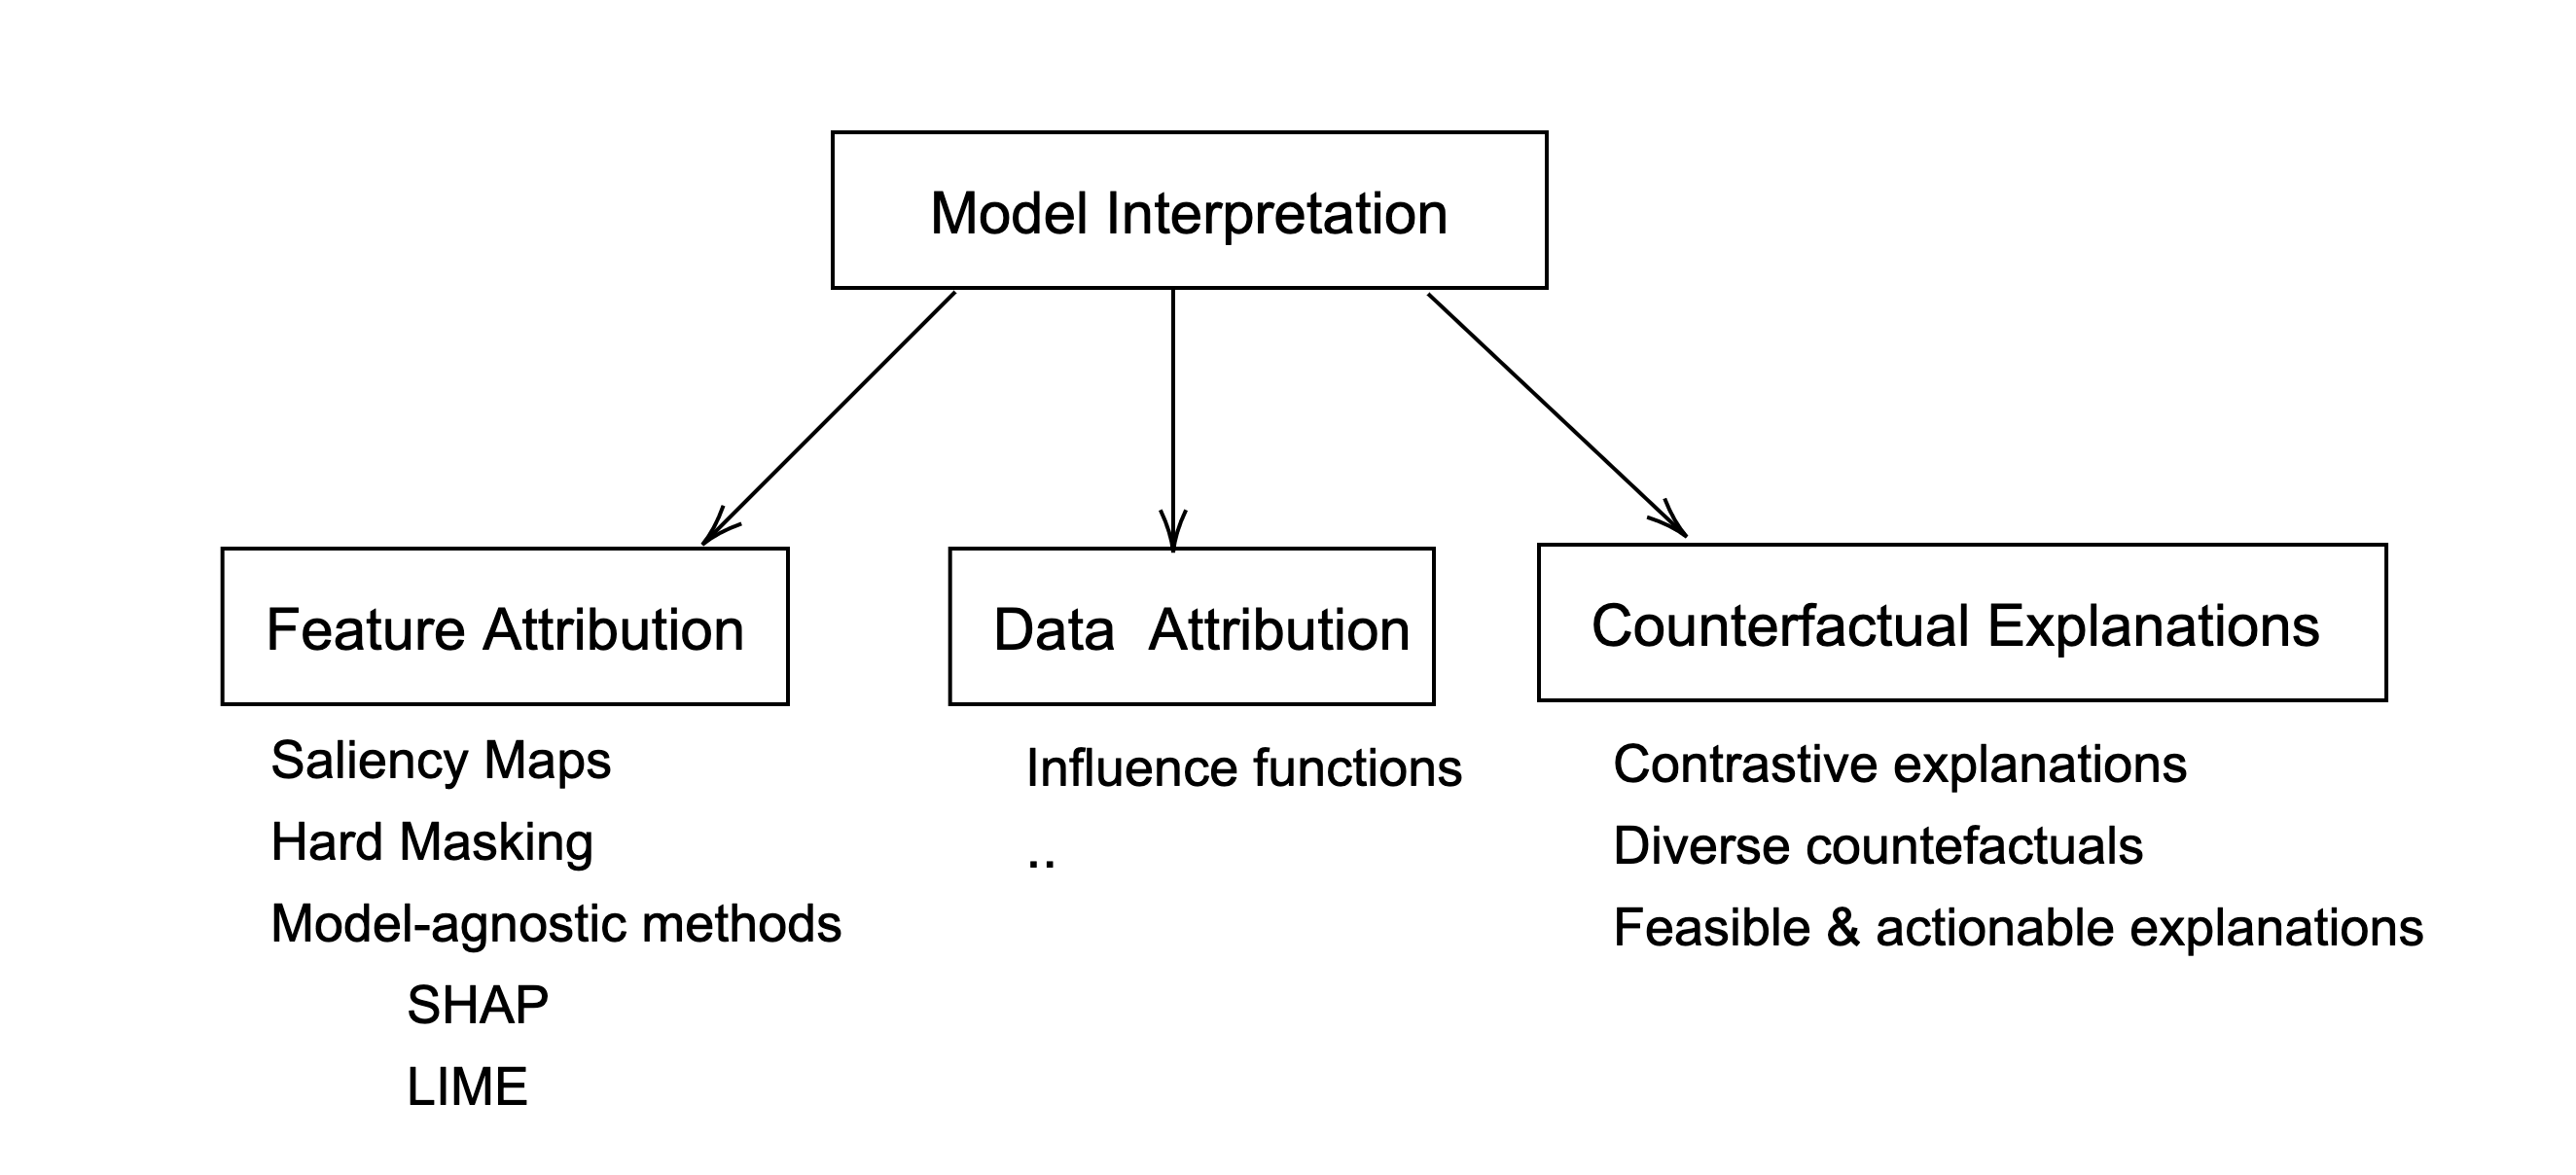
\includegraphics[width=\textwidth]{figure/1-attributions.png}
%     \end{center}
    \begin{center}
        \begin{tikzpicture}[every path/.style={->,line width=0.35mm,thick},
                            every label/.append style={align=left, font=\footnotesize, text width=4cm}]
            \node[main node] (1) { Model Interpretation };
            \node[main node,
                label={below:
                \tab[0.5cm] - Saliency Maps\\ %\tab[0.5cm] - Hard Masking \\
                \tab[0.5cm] - Model-agnostic methods \\ 
                \tab - SHAP\\ 
                \tab - LIME}
                ] (2) [below left = 1.3cm and 1.5cm of 1]  { Feature Attribution };
            \node[main node, text width=3cm, align=center,
                label={below: \tab[0.5cm] - Influence Functions\\ \tab[0.5cm] - ... }
                ] (3) [below = 1.3cm of 1] { Data Attribution };
            \node[main node,
                label={below:
                - Contrastive explanations\\ 
                - Diverse counterfactuals \\ 
                - Feasible \& actionable explanations}
                ] (4) [below right = 1.3cm and 1.5cm of 1] { Counterfactual Explanations };
            \draw (1) -- (2);
            \draw (1) -- (3);
            \draw (1) -- (4);
    
        \end{tikzpicture}  
    \end{center}
\end{frame}



% \begin{frame}{Types of Explanations}

% 	The output of an interpretation technique is an \textbf{explanation}, which can be of different types:

%     \medskip

% 	\begin{itemize}
%   \itemsep1em
% 	\item
% 		\textbf{Feature attribution:} Produce explanations on a per-feature level, \\
% 		e.g., feature effects or feature importance
% 		%Identifies (a subset of) features that are most responsible for a decision.
% 		\\
% 		%Input: feature $\rightarrow$ Output: target
% 		$\leadsto$ Vary feature values, inspect how model prediction, model variance or model error changes
% \pause
% 	\item
% 		\textbf{Data attribution:}
% 		Identify training instances that are most responsible for a decision
% \pause
% 	\item
% 	   \textbf{Counterfactual explanations:}
% 	   Identify smallest necessary change in feature values so that a desired outcome is predicted
% 	   \\
% 		%\smallskip
% 		%Input: target $\rightarrow$ Output: feature
% 		%Vary target, identify how feature needs to be changed

% 	\end{itemize}

% \end{frame}



% \begin{frame}{Feature Effects vs. Feature Importance}
% 
% 	\textbf{Feature Effects} indicate the change in prediction due to changes in feature values.
% 	\medskip
% 	\begin{center}
% 		\includegraphics[page=1, width=0.7\textwidth, trim=0 0 215 0, clip]{figure/feature-effect}
% 	\end{center}
% 	\begin{itemize}
% 		\item Model-agnostic methods: ICE curves, PD plots $\hdots$
% 		\item Pendant in linear models: Regression coefficient $\beta_j$
% 	\end{itemize}
% \end{frame}
% 
% \begin{frame}{Feature Effects vs. Feature Importance}
% 
% 	\textbf{Feature importance} methods rank features by how much they contribute to the predictive performance or prediction variance of the model.
% 	\begin{center}
% 		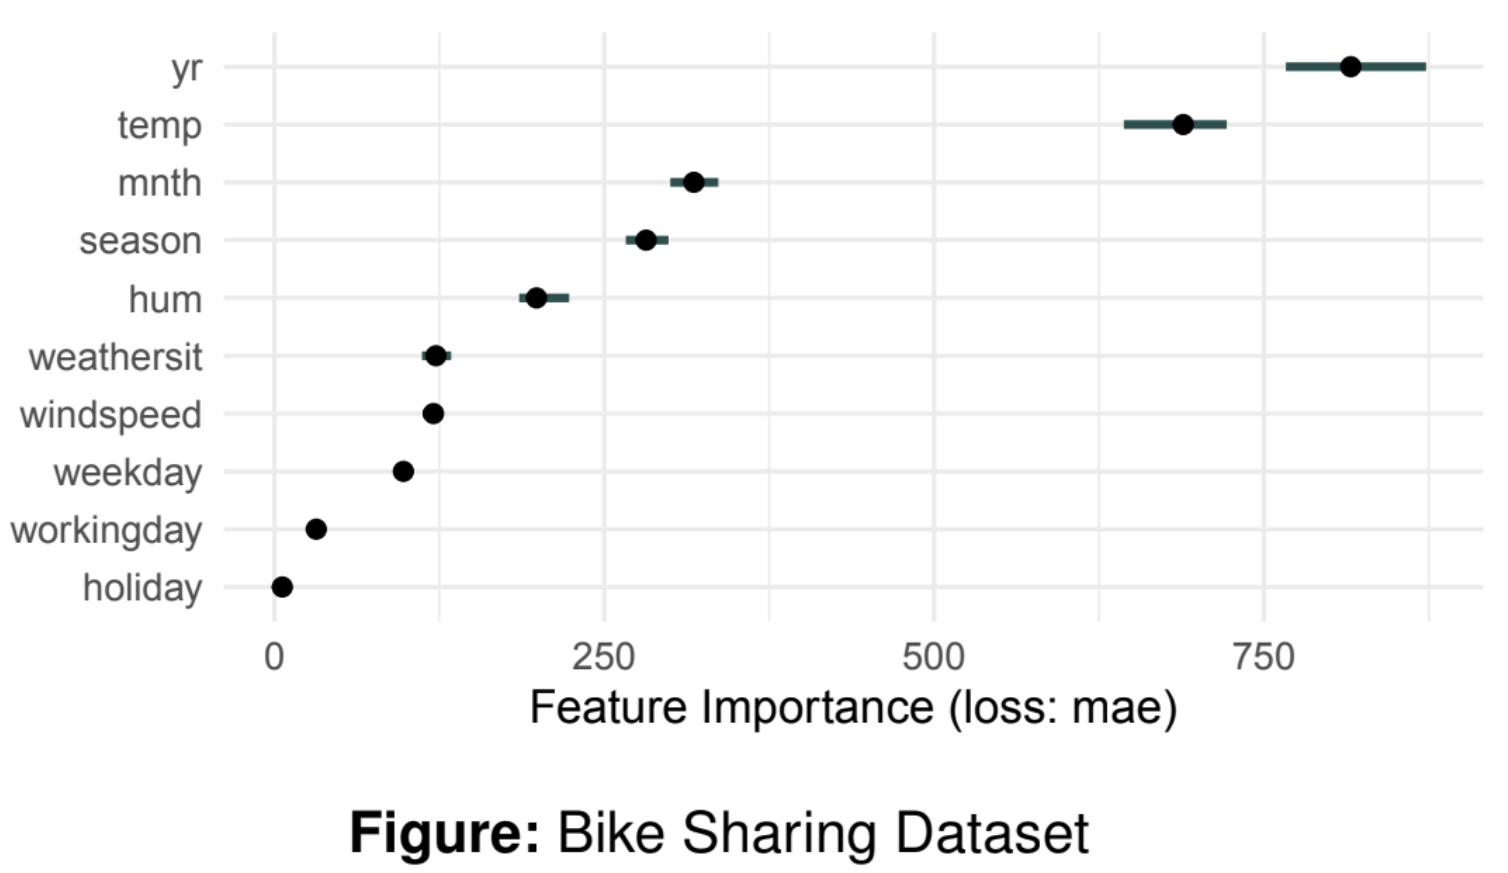
\includegraphics[page=1, width=0.4\textwidth]{figure/feature-importance}
% 	\end{center}
% 	\begin{itemize}
% 		%\itemsep1em
% 		\item Model-agnostic methods: PFI, $\hdots$
% 		\item Pendant in linear models: t-statistic, p-value (significant effect)
% 	\end{itemize}
% 
% \end{frame}
% 
% 
% \begin{frame}{Explanation using training instances~\citebutton{Koh et al. 2017}{https://arxiv.org/pdf/1703.04730.pdf}}
% 
% 	\textbf{Data attribution:} Which training instances results in the decision for the instance $x$ of the model?
% 	\begin{center}
% 		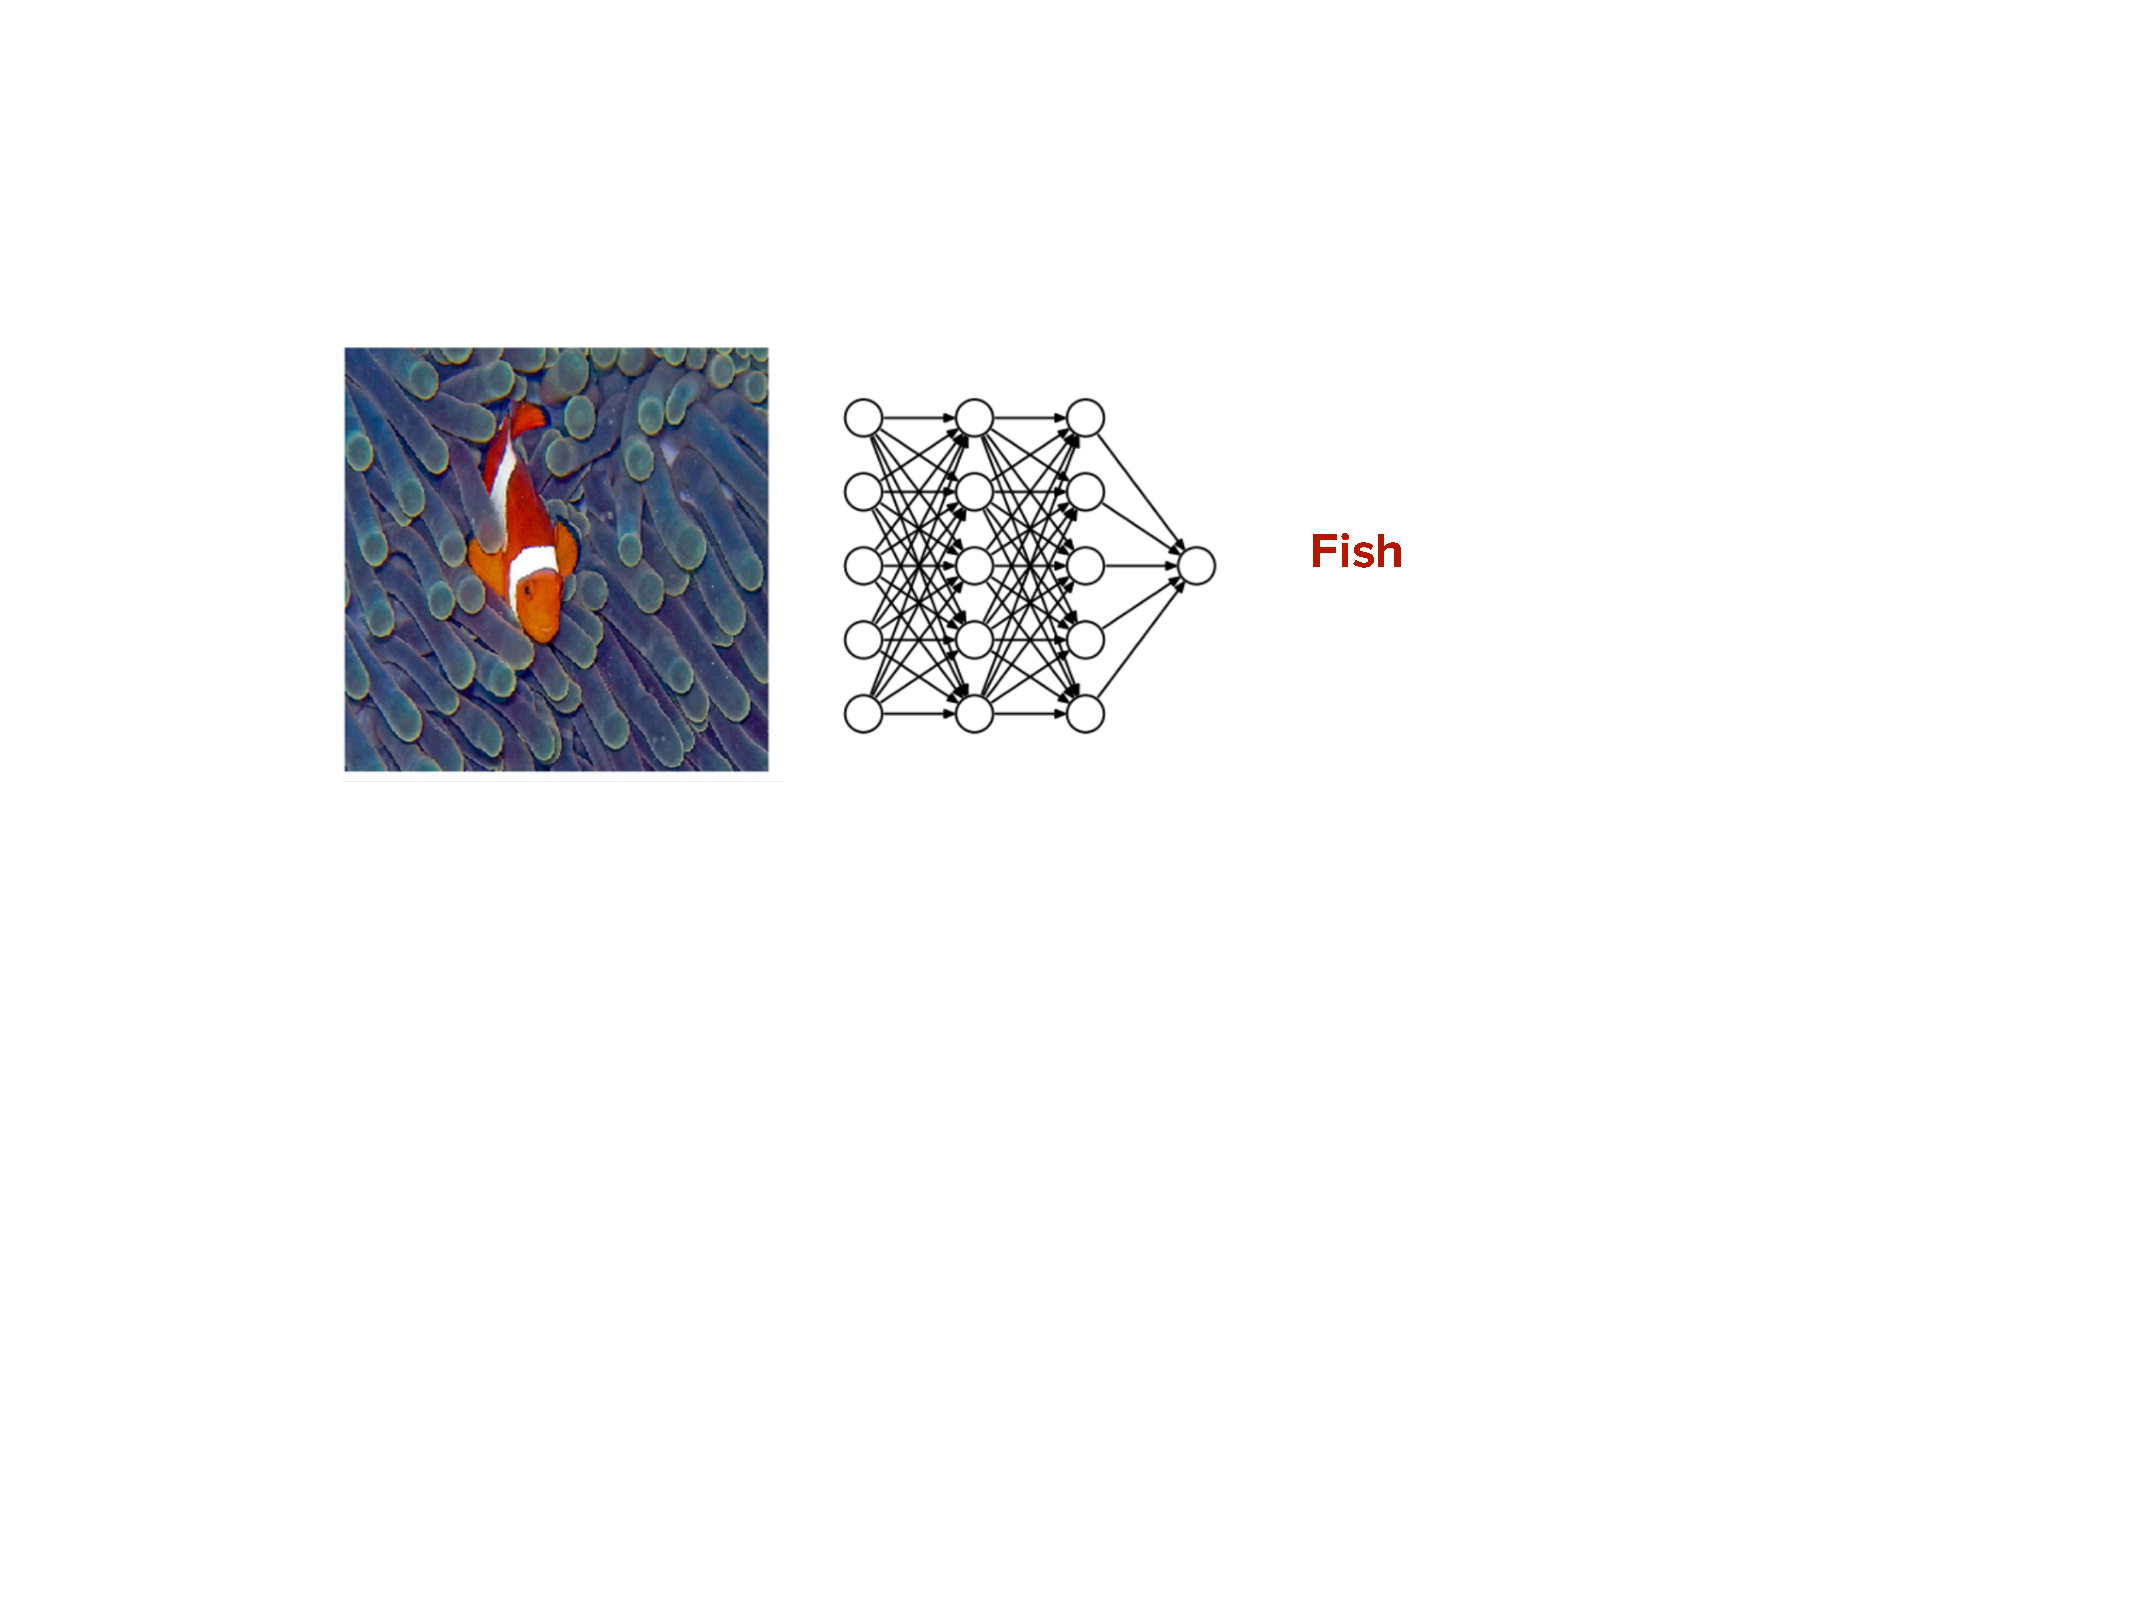
\includegraphics[page=1, width=0.7\textwidth]{figure/fish-attribution.pdf}
% 	\end{center}
% \end{frame}
% 
% \begin{frame}{Explanation using training instances~\citebutton{Koh et al. 2017}{https://arxiv.org/pdf/1703.04730.pdf}}
% 	\textbf{Data attribution:} Which training instances results in the decision for the instance $x$ of the model?
% 	\begin{center}
% 		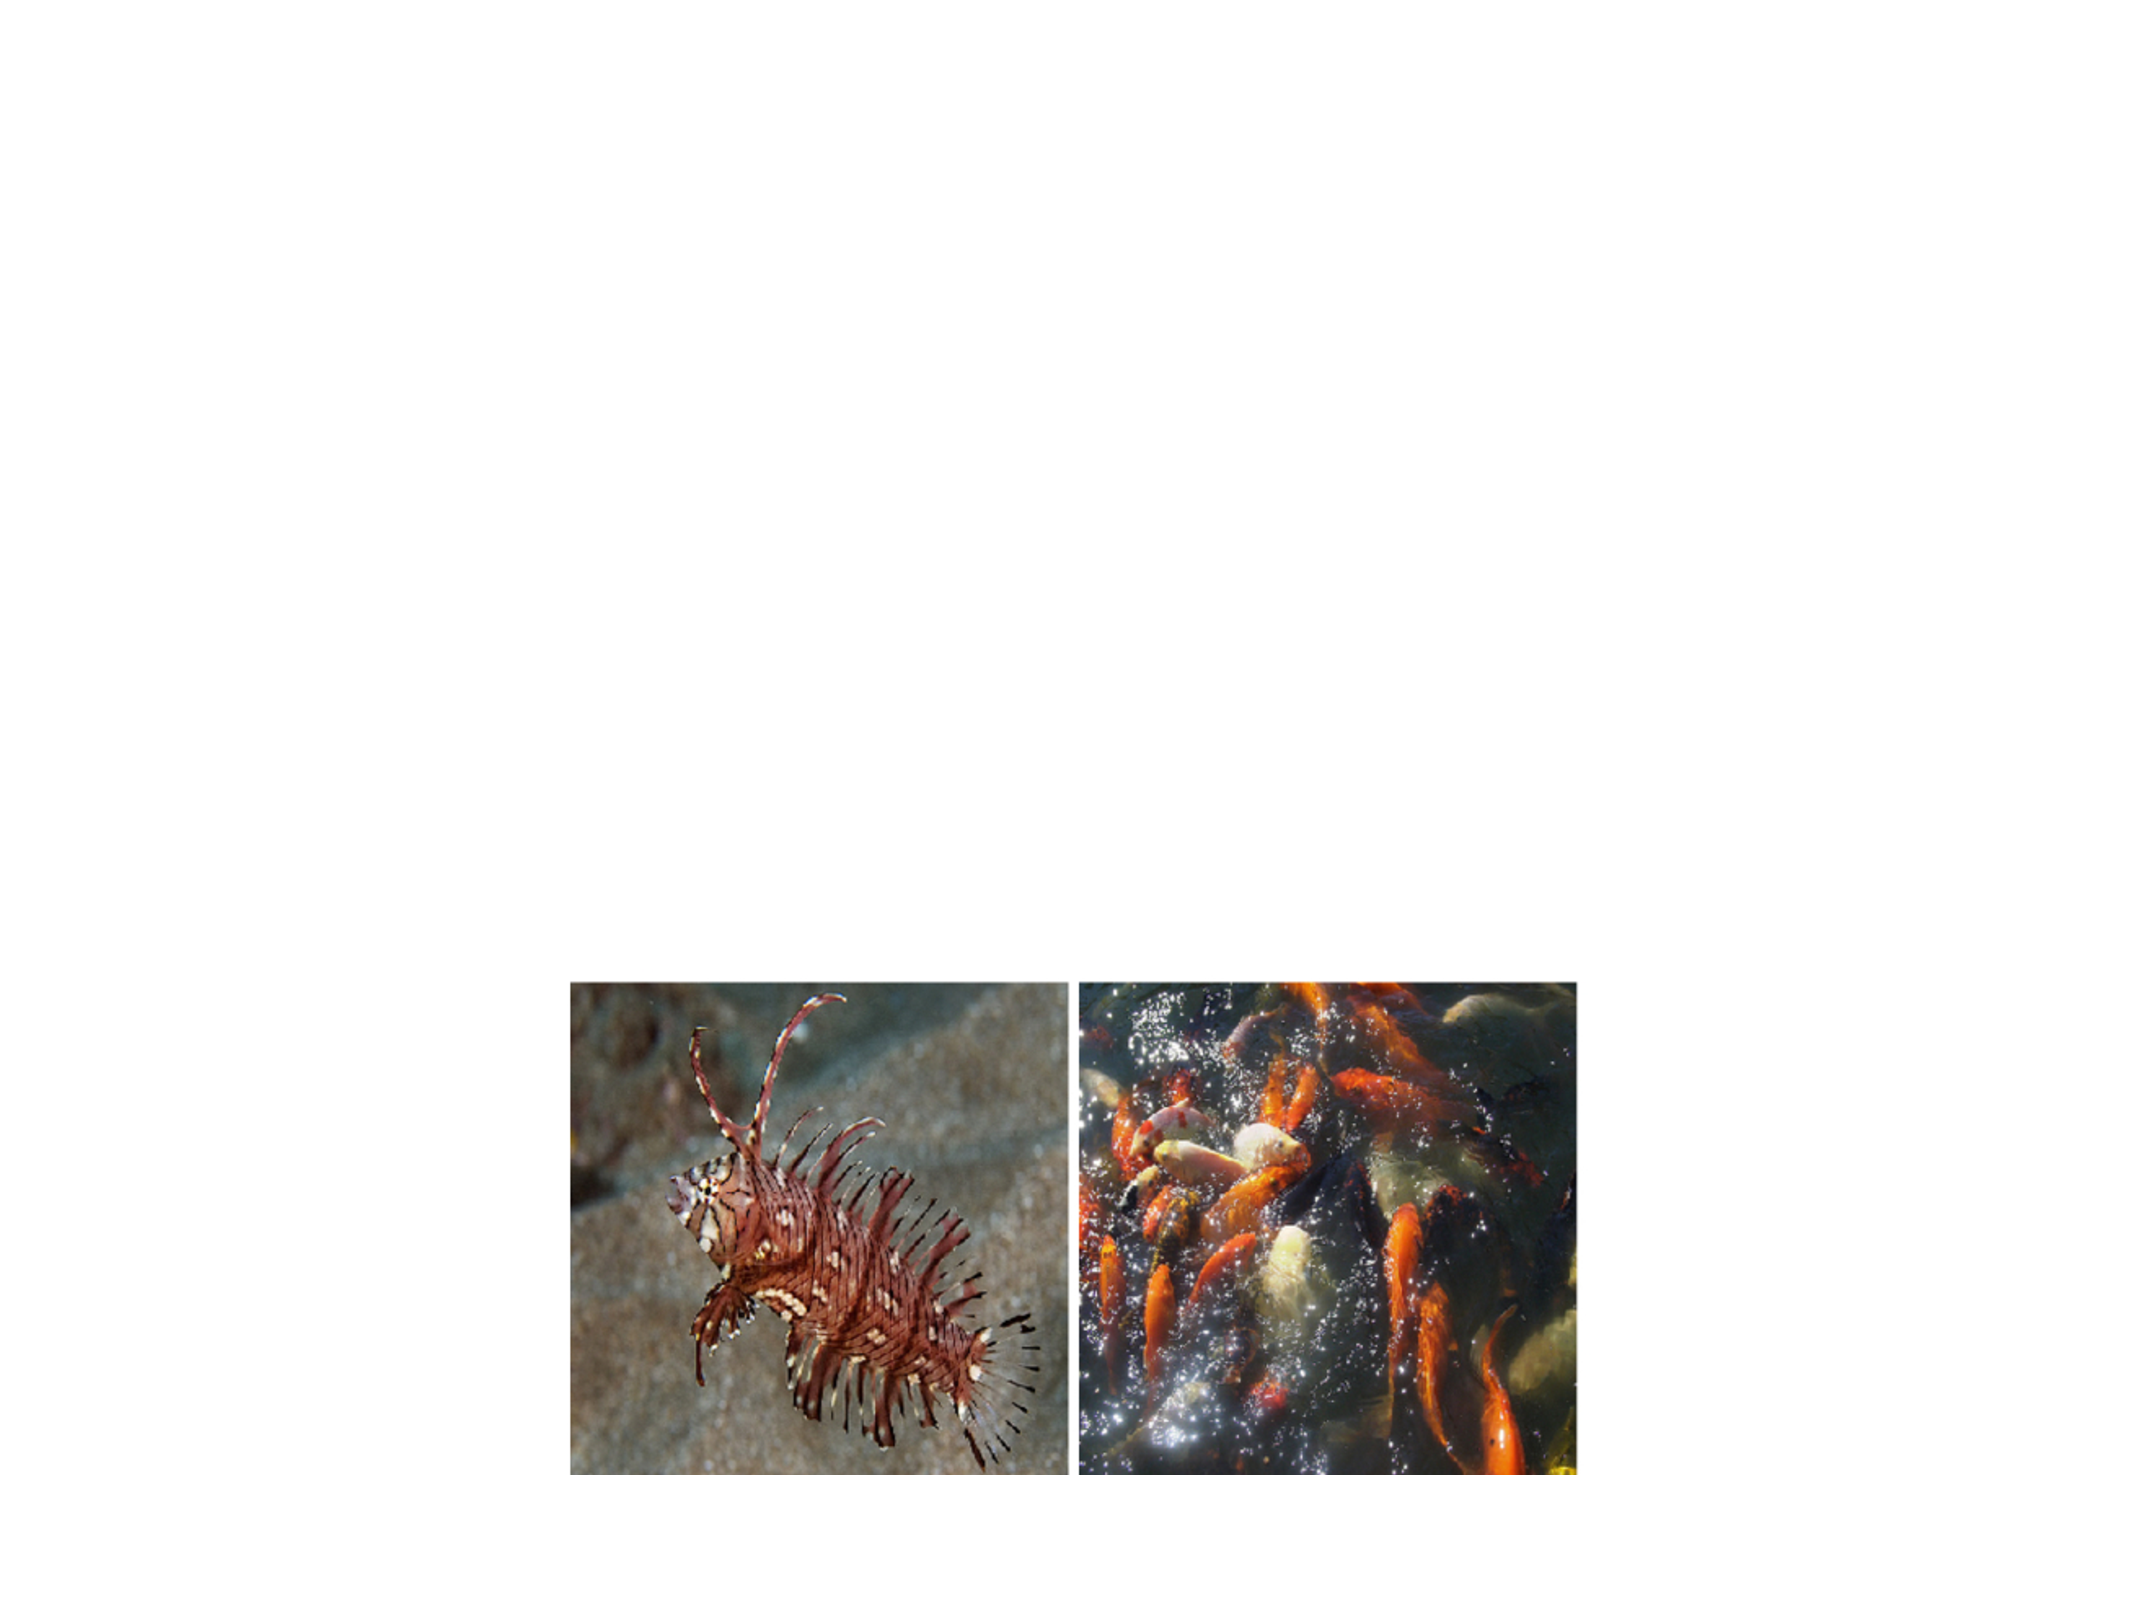
\includegraphics[page=1, width=0.7\textwidth]{figure/prototypes-fish.pdf}
% 	\end{center}
% 	\begin{itemize}
% 		\item Methods:
% 		Influence functions, prototype generation
% 	\end{itemize}
% \end{frame}
% 
% \begin{frame}{Explanation using Counterfactuals}
%     A counterfactual is small ``imperceptible'' change in $x$ causing a different prediction.\\
%     $\leadsto$ What if a small difference $ |x - x'| \leq \epsilon$ to $x$ causes a large change in the model output ?
%     
%     \textbf{Example} (loan application):
% 	\begin{center}
% 	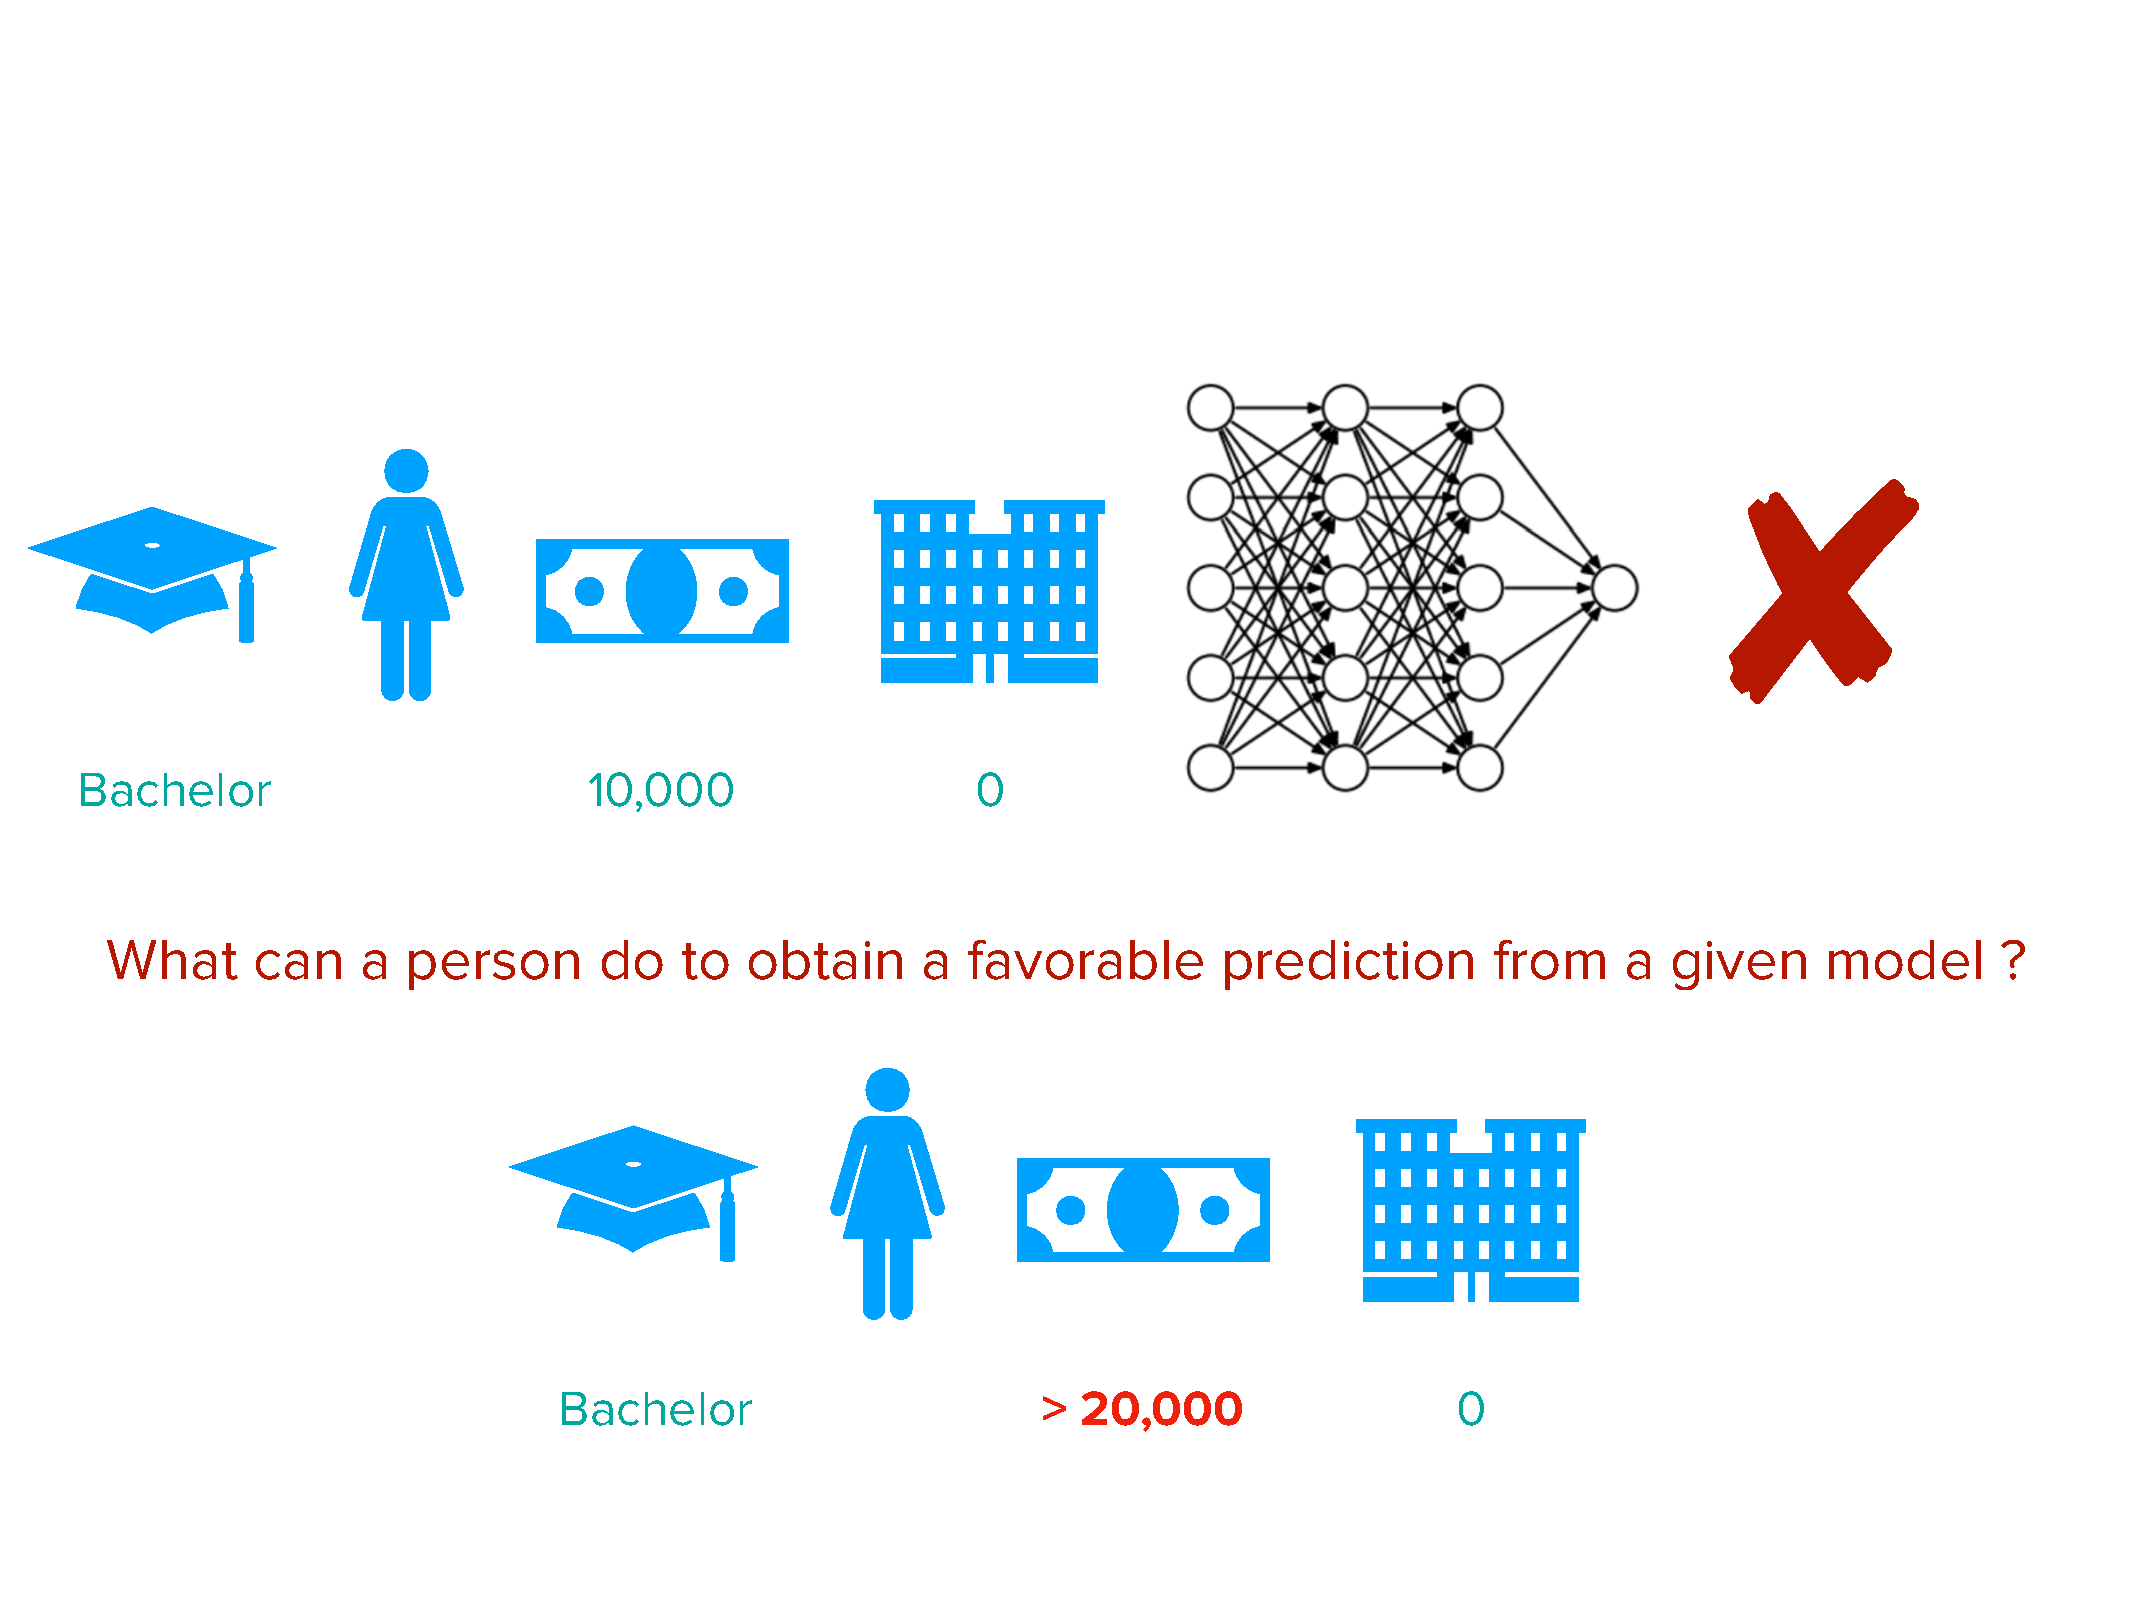
\includegraphics[page=1, width=0.7\textwidth]{figure/counterfactual.pdf}
% 	\end{center}
% 
% \end{frame}


\begin{frame}{Global vs. Local}
Global interpretation methods explain the model behavior for the entire input space by considering all available observations:
\begin{columns}[c, totalwidth=\textwidth]
    \begin{column}{0.65\linewidth}
	\begin{itemize}
		\item Permutation Feature Importance (PFI)
		\item Partial Dependence (PD) plots
		%\item Functional ANOVA (FANOVA)
		\item Accumulated Local Effect (ALE) plots
		\item ...
	\end{itemize}
\bigskip
Local interpretation methods explain the model behavior for single data instances:
	\begin{itemize}
		\item Individual Conditional Expectation (ICE) curves
		\item Local Interpretable Model-Agnostic Explanations (LIME)
		\item Shapley values, SHAP
		\item ...
	\end{itemize}
	\end{column}
	\begin{column}{0.35\linewidth}
	\begin{center}
	\includegraphics[page=1, width=0.7\textwidth, trim=215 0 215 43, clip]{../../slides/01_intro/figure/feature-effect}
	\medskip
	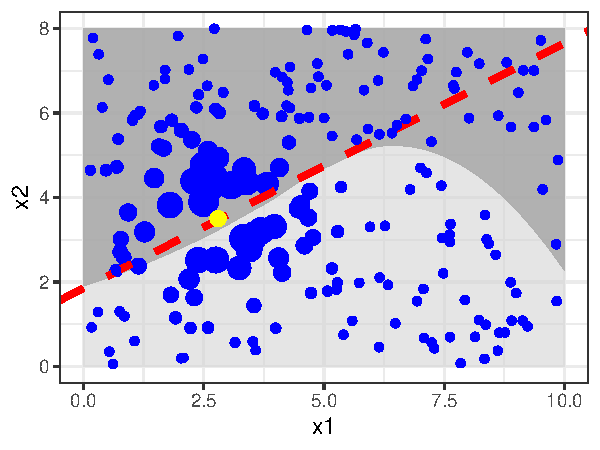
\includegraphics[width=0.7\textwidth]{../../slides/01_intro/figure/lime5}
	\end{center}
	\end{column}
	\end{columns}
\end{frame}

% \begin{frame}{Local vs. Global Explanations}
% % 	\begin{center}
% % 		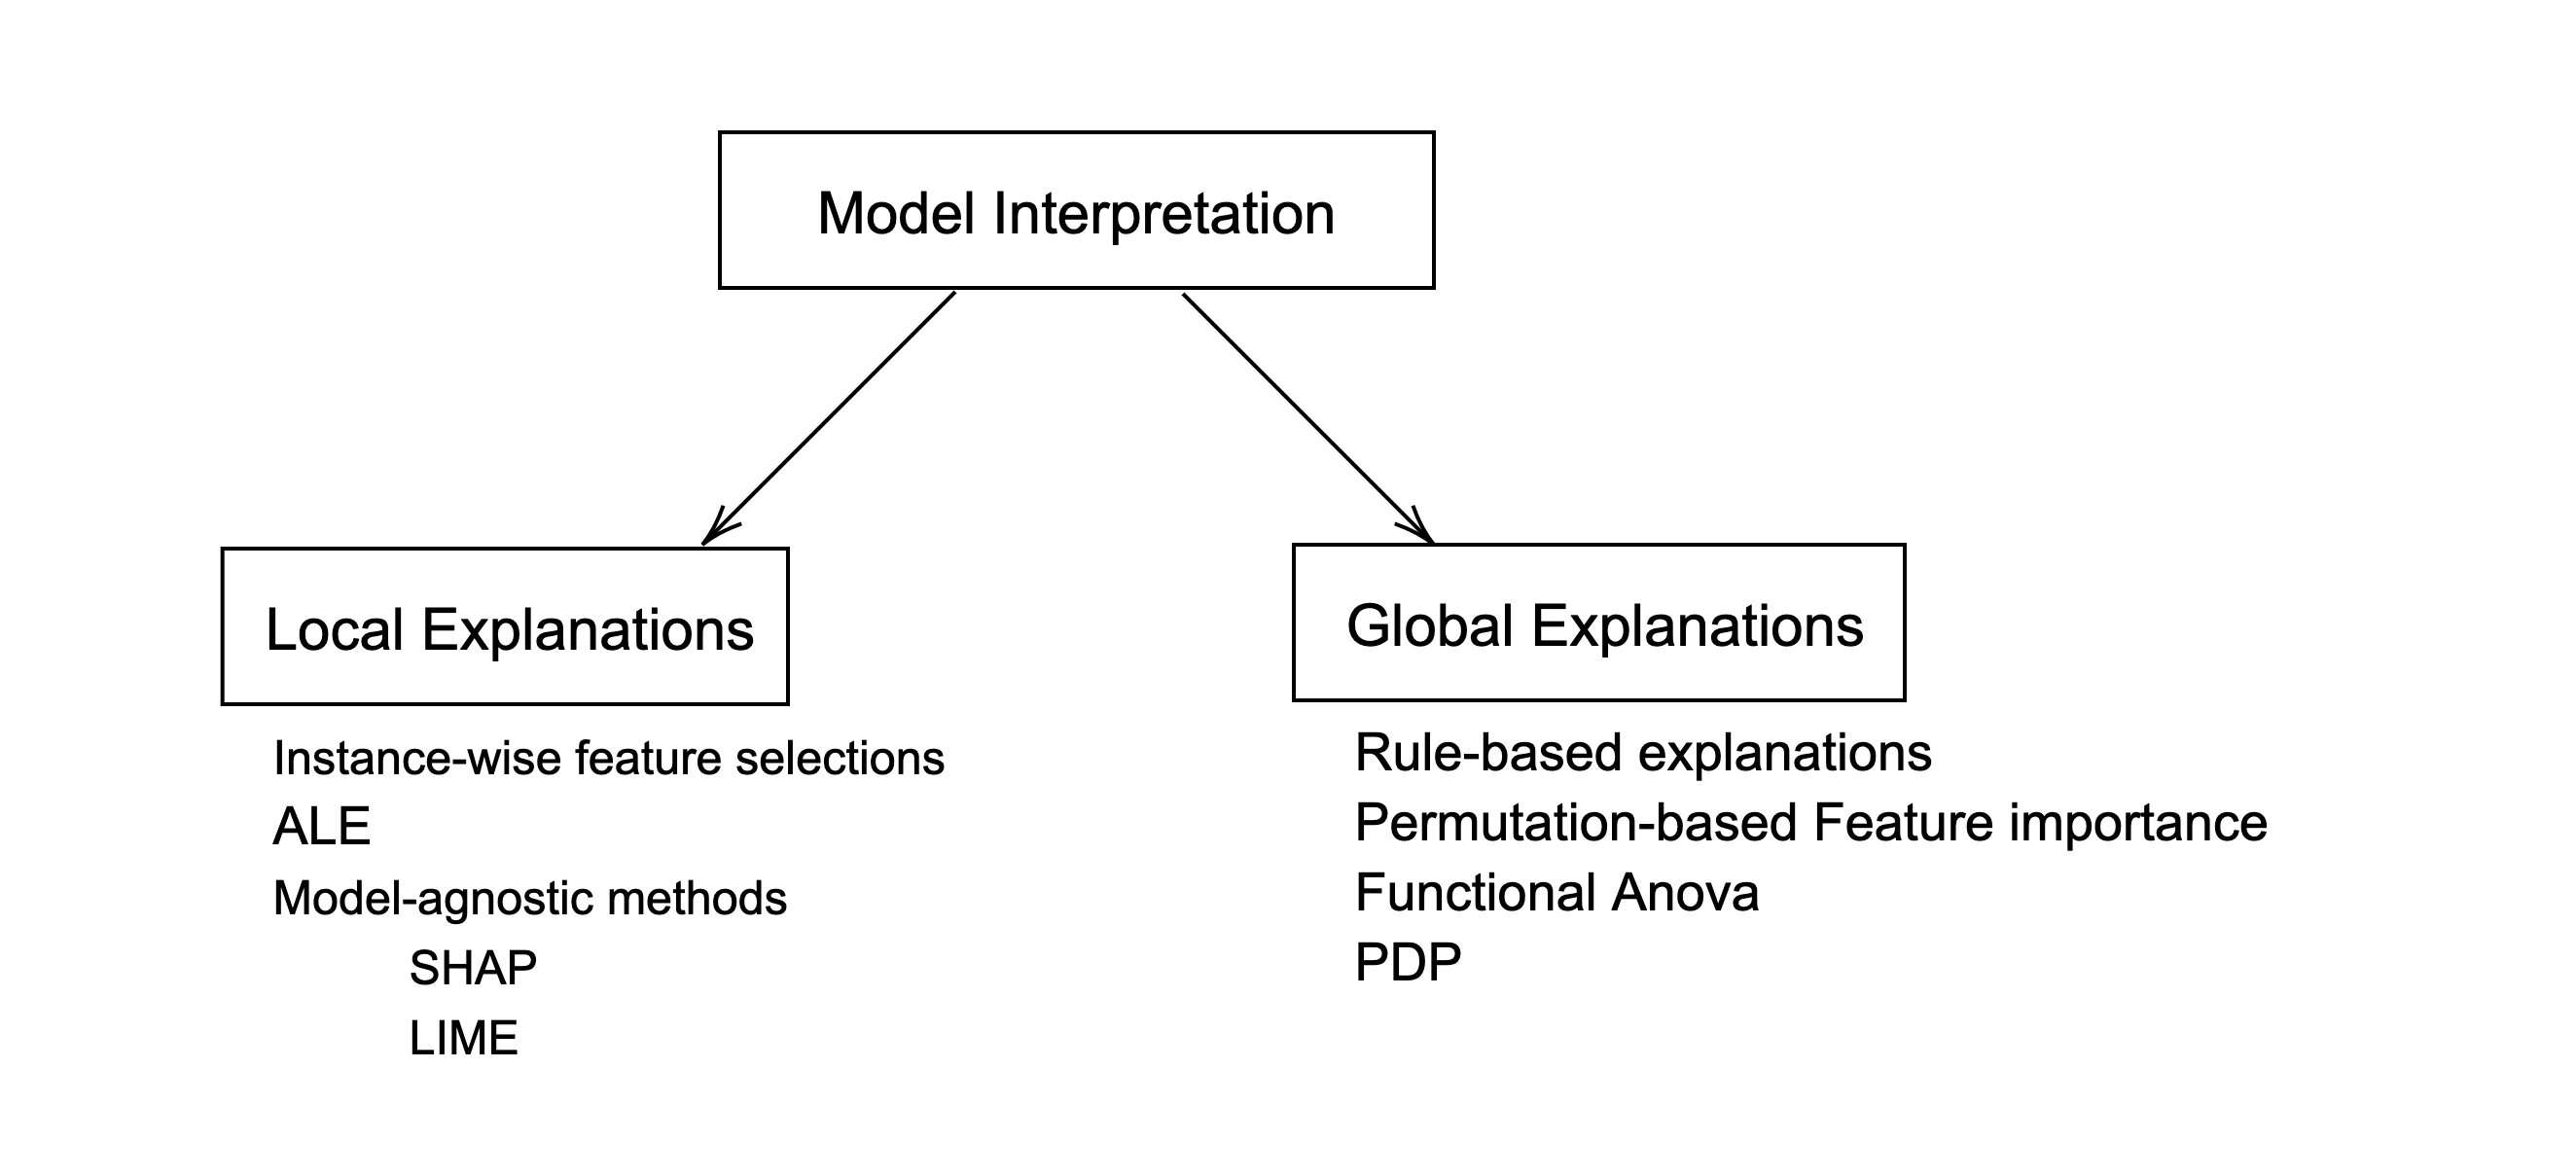
\includegraphics[width=\textwidth]{figure/1-local-global.png}
% % 		%TODO: Remove ALE from local
% % 	\end{center}

% \begin{center}
%     \begin{tikzpicture}[every path/.style={->,line width=0.35mm,thick},
%                         every label/.append style={align=left, font=\footnotesize, text width=6cm}]
%         \node[main node, text width=4cm, align=center] (1) { Model Interpretation };
%         \node[main node, text width=4cm, align=center, 
%             label={below:
%             \tab - Instance wise feature selections \\ 
%             \tab - Model-agnostic methods \\ \tab[1.5cm] - SHAP\\ 
%             \tab[1.5cm] - LIME}
%             ] (2) [below left = 1.3cm and 0cm of 1]  { Local Explanations };
%         \node[main node,  text width=4cm, align=center, 
%             label={below:
%             %Rule-based Explanations\\ 
%             \tab - Permutation feature importance \\ 
%             \tab - Functional ANOVA \\ 
%             \tab - PDP}
%             ] (3) [below right = 1.3cm and 0cm of 1] { Global Explanations };
%         \draw (1) -- (2);
%         \draw (1) -- (3);

%     \end{tikzpicture}  
% \end{center}
% \end{frame}


% \begin{frame}{Fixed Model vs. Refits}
% 	\begin{itemize}
% 		\itemsep1em
% 		\item Most methods we will discuss analyze a fixed, trained model (e.g., PD plots, PFI)
% 		\item Some methods require refitting of the model (e.g., PIMP)
% 		\item Trained model $\Rightarrow$ Model is the object of analysis
% 		\item Refitting $\Rightarrow$ Learning process is the object of analysis
% 		\item Advantage of refitting: It includes information about the variability in the learning process
% 	\end{itemize}
% \end{frame}


% \begin{frame}{Intrinsic and Model-Agnostic Interpretation}
% \begin{itemize}
%   \item Intrinsically interpretable models:
%   \begin{itemize}
%   \item Examples are linear models and decision trees.
%   \item They are interpretable because of their simple structures, e.g.,
%   a weighted combination of feature values or a tree structure.
%   \item However, they are difficult to interpret with many features or complex interaction terms.
%   \end{itemize}
%   \lz
%   \item Model-agnostic interpretation methods:
%   \begin{itemize}
%   \item They are applied after training (post-hoc).
%   \item They also work for more complex black box models.
%   \item They can also be applied to intrinsically interpretable models, e.g.
%     feature importance for decision trees.
%   \end{itemize}
% \end{itemize}
% \end{frame}
%
% \begin{frame}{Model-Agnostic Interpretability}
%  \begin{itemize}
%   %\itemsep2em
%   \item Model-agnostic interpretability methods work for \textbf{any} kind of machine learning model.
%   \item Explanation type is not tied to the underlying model type.
%   \item Often, only access to data and fitted predictor is required. No further knowledge about the model itself is necessary.
%   \item We usually distinguish between \textbf{feature effect} and \textbf{feature importance} methods.
%  \end{itemize}
% \end{frame}
%
%
% \begin{frame}{Feature Effects vs. Feature Importance}
% \textbf{Feature effects} indicate the direction and magnitude of a change in predicted outcome due to changes in feature values.
% \begin{center}
% \includegraphics[page=1, width=\textwidth]{figure/feature-effects}
% \end{center}
%   \begin{itemize}
%     \item Methods include: Partial Dependence Plots, Individual Conditional Expectation, Accumulated Local Effects (ALE)
%     \item Pendant in linear models: Regression coefficient $\hat{\theta}_j$
%   \end{itemize}
% \framebreak
%
% \textbf{Feature importance} methods rank features by how much they contribute to the predictive performance or prediction variance of the model.
% \begin{columns}
% \begin{column}{0.6\textwidth}
% \begin{itemize}
%     %\itemsep1em
%     \item Methods include: Permutation Feature Importance, Functional Anova
%     \item Analog in linear models: Absolute t-statistic $\left|\frac{\hat{\theta}_j}{SE(\hat{\theta}_j)}\right|$
% \end{itemize}
% \end{column}
% \begin{column}{0.4\textwidth}
% \begin{center}
% 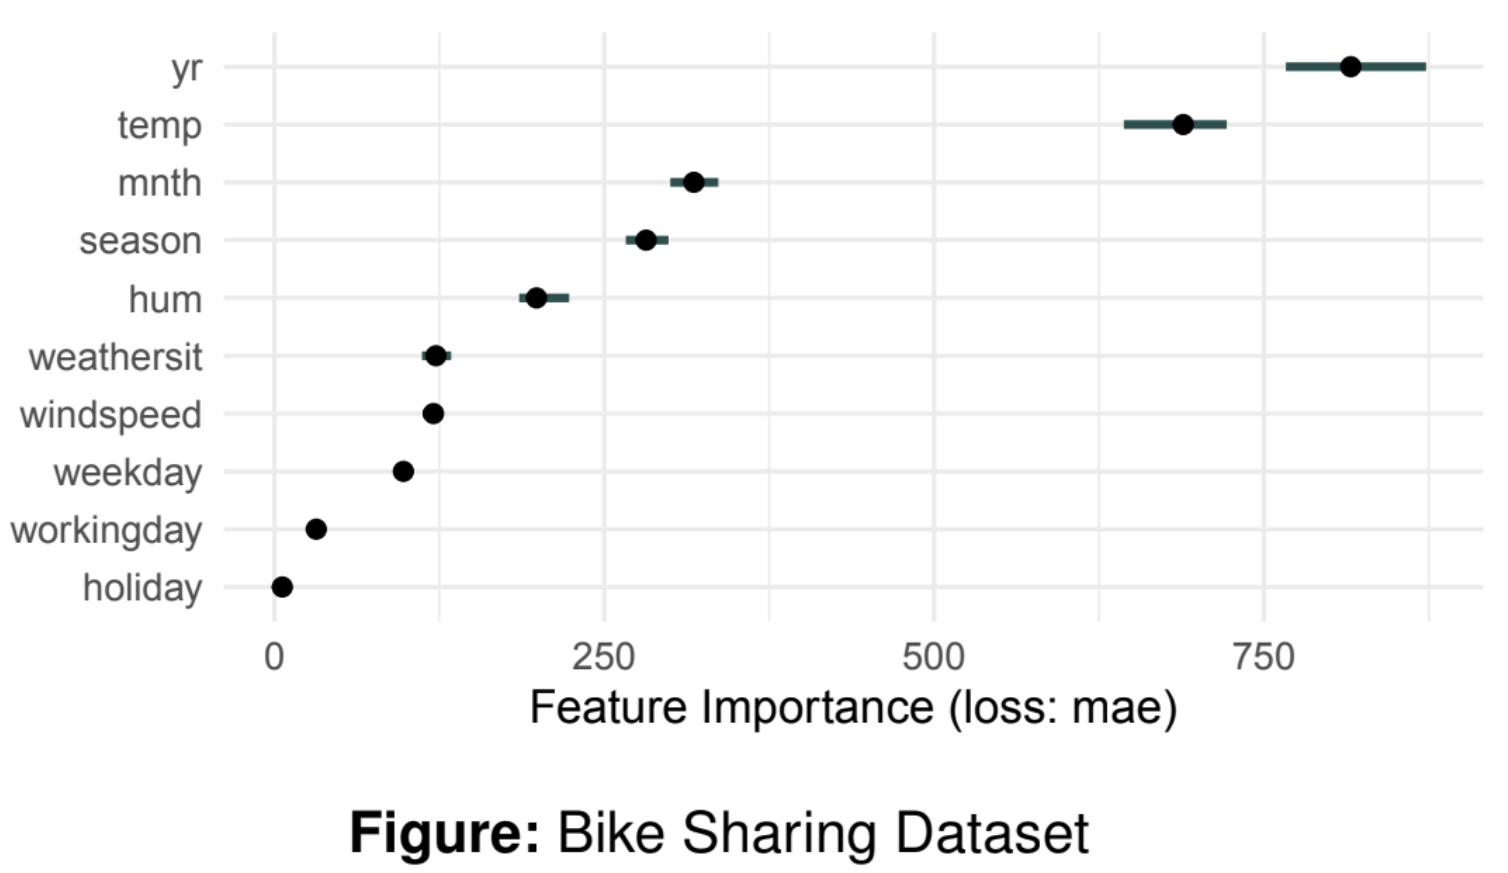
\includegraphics[page=1, width=\textwidth]{figure/feature-importance}
% \end{center}
% \end{column}
% \end{columns}
% \end{frame}
%
%
% \begin{frame}{Global and Local Interpretability}
% Global interpretability methods explain the expected model behavior for the entire feature space by considering all available observations (or representative subsets). For example:
%   \begin{itemize}
%     \item Permutation Feature Importance
%     \item Partial Dependence Plot
%     \item Functional Anova
%     \item ...
%   \end{itemize}
% \lz
% Local interpretability methods explain single predictions or a group of similar observations. For example:
%  \begin{itemize}
%   \item Individual Conditional Expectation (ICE) Plots
%   \item Local Interpretable Model-Agnostic Explanations (LIME)
%   \item Shapley Values
%   \item ...
%  \end{itemize}
% \end{frame}
%
%
% \begin{frame}{Fixed model vs. refits}
%   \begin{itemize}
%      %\itemsep2em
%      \item Most methods presented in this lecture analyze a fixed, trained model
%      (e.g., permutation feature importance).
%      \item Some methods require refitting the model (e.g., PIMP).
%      \item Trained model $\Rightarrow$ Model is the object of analysis.
%      \item Refitting $\Rightarrow$ Learning process is the object of analysis.
%      \item The advantage of refitting is that it includes information about the variability in the learning process.
%   \end{itemize}
% \end{frame}


% \endlecture
% 
% 
% 
% \lecturechapter{Bike Sharing Dataset}
% \lecture{Interpretable Machine Learning}

\begin{frame}[t]{Bike Sharing Dataset \citebutton{Fanaee-T and Gama (2014)}{https://doi.org/10.1007/s13748-013-0040-3}}
\begin{itemize}
\item Daily counts of rented bikes in Washington D.C. from \citebutton{Capital-Bikeshare}{https://capitalbikeshare.com/}
\item Feature description:
\begin{itemize}
\item \code{cnt}: count of total rental bikes (prediction target for regression)
\item \code{season}: season (1: WINTER, 2: SPRING, 3: SUMMER, 4: FALL)
\item \code{yr}: year (0: 2011, 1: 2012)
\item \code{mnth}: month of year (1: JAN, ..., 12: DEC)
\item \code{holiday}: day is holiday (0: NO HOLIDAY, 1: HOLIDAY)
\item \code{weekday}: day of the week (1: SUN, 2: MON, ..., 7: SAT)
\item \code{workingday}: day is not a weekend or holiday (0: NO WORKING DAY, 1: WORKING DAY)
\item \code{weathersit}: weather situation (1: GOOD, 2: MISTY, 3: RAIN/SNOW/STORM)
\item \code{temp}: temperature in Celsius
\item \code{hum}: humidity in percent
\item \code{windspeed}: wind speed in km/h
\item \code{days\_since\_2011}: Number of days since January 1st, 2011 (start of historical log)\\
$\leadsto$ accounts for the trend over time
\end{itemize}
\end{itemize}
\end{frame}


\begin{frame}[t]{Bike Sharing Dataset - EDA}
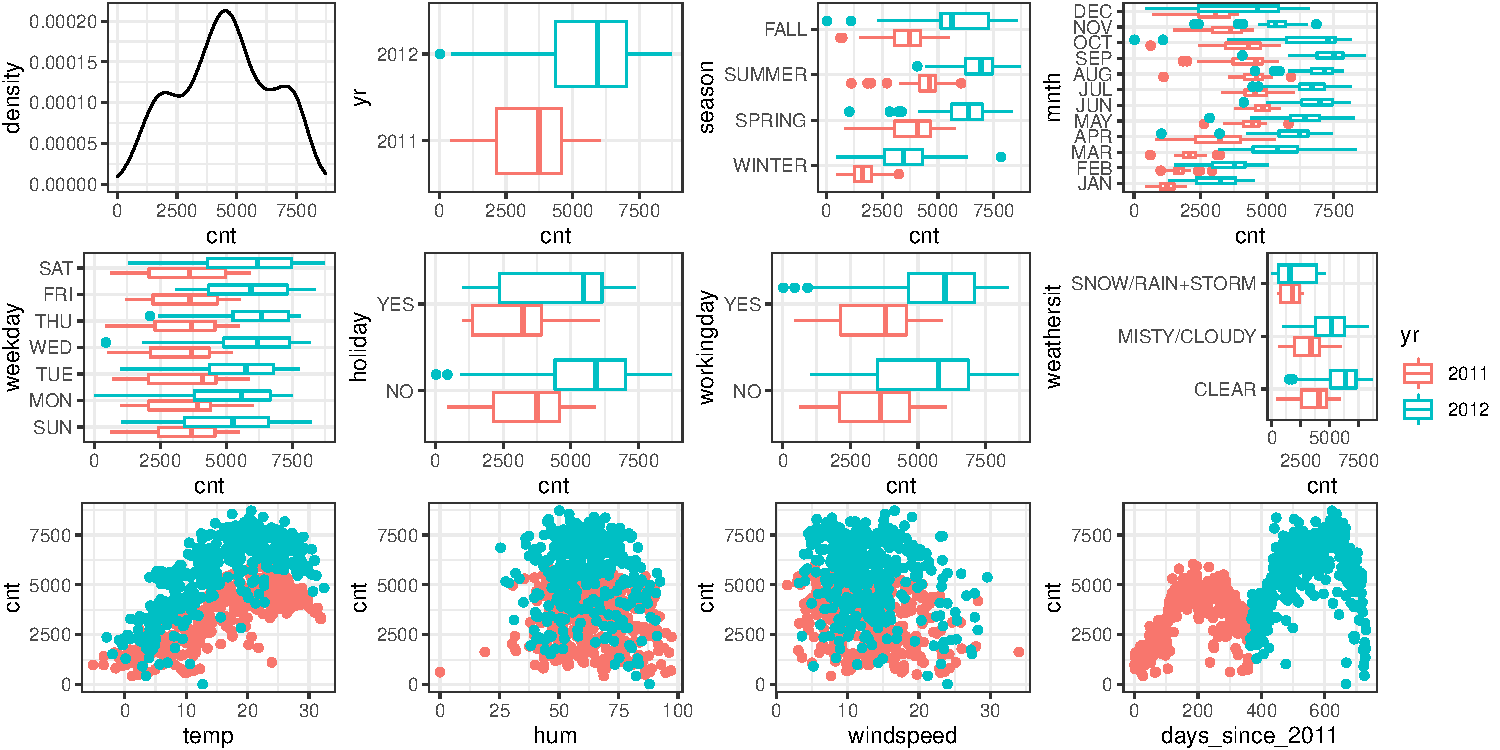
\includegraphics[width=\linewidth]{../../slides/01_intro/figure/intro_bike}
\end{frame}

\endlecture

\end{document}



 